\documentclass[12pt,a4paper,titlepage]{article}
\usepackage[utf8]{inputenc}
\usepackage[T1]{fontenc}
\usepackage{amsmath}
\usepackage{amsfonts}
\usepackage{amssymb}
\usepackage[left=3cm,right=3cm,top=2.5cm,bottom=2.5cm]{geometry}
\usepackage[dvipsnames]{xcolor}
\usepackage[czech]{babel}
\usepackage[
  backend=biber,
  style=iso-numeric,
  maxbibnames=99
]{biblatex}
\addbibresource{maturitni_prace.bib}
\usepackage{graphicx}
\usepackage{minted}
\usepackage{subcaption}
\usepackage{tikz}
\usepackage{pgfplots}
\pgfplotsset{compat=1.18}
\graphicspath{ {./images/} }
\usepackage{indentfirst}
\usepackage{setspace}
\fontfamily{ptm}
\usepackage{tabularx,ragged2e,booktabs}
\usepackage{hyperref}
\usepackage{csquotes}
\usepackage{xurl}

\DeclareBibliographyCategory{skipbibliography}
\DeclareCiteCommand{\fcite}[\mkbibfootnote]
  {\usebibmacro{prenote}}
  {\addtocategory{skipbibliography}{\thefield{entrykey}}%
   \usedriver{\DeclareNameAlias{sortname}{default}}{\thefield{entrytype}}}
  {\multicitedelim}
  {\usebibmacro{postnote}}

\author{Antonín Vřešťál}
\title{Tvorba astronomických videí}
\renewcommand{\baselinestretch}{1.5} 


\begin{document}
\begin{titlepage}
	\begin{center}
		Waldorfská základní a~střední škola Semily, p.\  o.\\
		Tyršova 485, 513 01 Semily
		\vspace*{1cm}
 
		\vfill		

		\Huge
		Tvorba astronomických videí
 
		\normalsize
		\vspace{0.5cm}
		Maturitní práce 	 
		 
		\vfill		
	\end{center}
	Vypracoval: Antonín Vřešťál\\
	Vedoucí práce: MgA. Mojmír Dlabola\\
	\textcolor{red}{Pracovní verze}\\
 \end{titlepage}
\newpage
\section*{Prohlášení}
Prohlašuji, že jsem tuto projektovou maturitní práci \enquote{Tvorba astronomických videí} napsal samostatně a~výhradně s~použitím citovaných pramenů. Souhlasím, aby má projektová maturitní práce byla zpřístupněna veřejnosti ke studijním účelům.
\section*{Poděkování}
Děkuji MgA. Mojmíru Dlabolovi, vedoucímu mé práce, za podnětné připomínky k~projektové maturitní práci po stránce obsahové i~stylistické a~za doporučení vhodné a~zajímavé literatury. Velmi si vážím času, který věnoval vedení mé práce.\\
\\
V Semilech dne \hspace{0.05cm} \rule[-3pt]{1.5in}{0.5pt}\\
\\
\hspace{0.5cm} \rule[-3pt]{5.5cm}{0.5pt}\\
\indent \indent Antonín Vřešťál\\

\newpage
\tableofcontents
\newpage
\part{Teoretická část}
\section{Úvod}
%\textcolor{red}{(Nejsem si úplně jistý, jak by měla tato sekce vypadat, budu rád za Váš názor.)}
Tvorbou astronomických videí se zabývám více než tři roky, a~to jako editor ve skupině AstroCrew. Skupinu AstroCrew tvoří tři členové:

\begin{itemize}
	\item Daniel Kurtin píše scénáře,
	\item Terka Toušová načítá text na mikrofon
	\item Já (Antonín Vřešťál) k~nahrávkám následně tvořím grafický podklad a~kompletuji veškerá data do výsledného videa.
\end{itemize}
Hotová videa následně publikujeme na našem YouTube kanálu. 

Základním cílem skupiny AstroCrew je zpřístupnit široké veřejnosti zajímavé úkazy na obloze pomocí animací a~videí. Diváci mají poté lepší přehled o~umístění jednotlivých úkazů na noční obloze a~mohou je následně lépe nalézt.

Spolupracujeme s~planetáriem v~liberecké iQLandii. Na jejich akcích \enquote{Večery pod hvězdami} jsou naše nová videa promítána přímo v~planetáriu jako součást oficiálního programu. Kromě videí o~astronomii zpřístupňujeme široké veřejnosti i~kosmonautiku. V~tomto odvětví se věnujeme primárně živým přenosům startů raket, poslední dobou nejvíce programu Starship.

Téma tvorby astronomických videí jsem si vybral zejména kvůli jeho obsáhlosti. V~rámci produkce videí ve skupině AstroCrew programuji animační nástroje, ale následně pomocí nich animuji scénu a~výsledná data nakonec kompletuji ve finální video. V~této maturitní práci se zaměřuji zejména na moji část produkce videa. Ostatní části tvorby videa, které nezpracovávám já, jsou zastoupeny pouze stručně obsahově pro doplnění kontextu. 
\section{Postup vytváření videa}\label{makingof}
\subsection{Příprava textových podkladů}\label{makingof:text-prep}
Téma připravovaného videa je většinou rozhodnuto s~dostatečným předstihem na základě společném diskuze. Každé video je unikátní s~ohledem na námi zvolené požadavky. Tyto požadavky vybíráme na základě chyb, nedostatků a~nových zjištění nabytých při tvorbě předchozích videí. V~případě videa, týkajícího se úkazů na noční obloze v~roce 2025, byla hlavním tématem diskuze o~jeho délce s~ohledem na rozhodnutí, které úkazy do videa budou zahrnuty a~které bude nutno vynechat.

Dalším krokem v~produkci videa je sepsání scénáře naším scénáristou Danem Kurtinem. Scénář videa určuje, jak bude celé video navenek působit, jaké informace bude obsahovat a v jakém sledu a hlavně jakým způsobem budou tyto informace divákovi podány. I dobrý nápad může totiž rychle ztroskotat, pokud není promyšleno, jak bude tento nápad prezentován.

Do našich videí, která se zaměřují hlavně na úkazy na obloze, se dají podklady shánět v odborných článcích, na amatérských profilech na sociálních sítích nebo přímo v programech simulujících umístění objetků na noční obloze. Tyto programy, jako je například Stellarium, vytvářejí na základě vědeckých měřeních opravdu věrný obrázek budoucnosti. 

Tento fakt se nám hodí při našich videích, která mají shrnovat nejdůležitější úkazy v budoucím roce. V tomto případě vybíráme většinou patnáct až dvacet úkazů, které může pozorovat i úplný amatér a to většinou bez použití jakékoliv techniky. Dalším naším typickým obsahem videí je souhrn každoročního dění na obloze v jednotících měsících roku. Způsob vytváření scénáře je dost podobný v obou případech --- pokaždé chronologicky prezentujeme to, co bude vidět v noci na obloze.

Jsou samozřejmě úkazy, které se opakují pravidelně každý rok. To jsou například meteorické roje, letní noční svítící oblaka nebo třeba viditelnost zvířetníkového světla. Informace o těchto událostech jsou většinou snadno dohledatelné. Pokaždé je však nutné zjistit, zda v období, kdy k této události dojde, nebude na obloze rušit Měsíc. Ten totiž při meteorických rojích může úplně znemožnit pozorování. I na to je dobré diváka upozornit, protože viditelnost těchto úkazů se může rok od roku měnit.

Další kategorií jsou úkazy, které jsou poměrně běžné, ale neopakují se každý rok ve stejný čas. Někdy k nim zkrátka dojde a bez podrobnějších informací není možné vědět, kdy nastanou. Do této kategorie spadají například zatmění Slunce a Měsíce, přílety jasnějších komet nebo třeba opozice planet (období, kdy je určitá planeta z našeho pohledu na opačné straně než Slunce, a jeví se tak jasněji). Zmínku o těchto jevech můžeme najít již poměrně dopředu v různých odborných článcích, které nám dokáží významně usnadnit práci s hledáním. Z česko-slovenských webových stránek to může být jmenovitě třeba stránka \href{https://www.astro-novinky.eu}{astro-novinky.eu} a ze zahraničních například stránka \href{https://in-the-sky.org}{in-the-sky.org}, která obsahuje i velmi pěkně zpracovaný kalendář úkazů na několik let dopředu.

Existuje spousta krásných úkazů, o kterých se ale dopředu moc nepíše. Pro ně je často potřeba využít právě primární zdroj, kterým je většinou Stellarium. Úkolem je prohledat den po dni oblohu a najít zejména zajímavé konjunkce (zdánlivá přiblížení objektů) nebo zákryty hvězd nebo planet Měsícem.\@ 

Náš scénárista Daniel Kurtin mi k tvorbě scénáře řekl: \enquote{Začnu vždy tím, že si vyberu nějaký objekt. Typicky začínám Merkurem. Následně si zrychlím čas a pozoruji, jestli se Merkur nepřiblíží k nějaké jiné planetě nebo k Měsíci, či zda se dokonce nesetká s nějakým jasnějším objektem vzdáleného vesmíru, například nějakou hvězdokupou. Stejně postupuji i u zbylých planet a nakonec u Měsíce. Tento proces je skutečně užitečný, protože lze vždy nalézt navíc něco, o čem jsem před tím ještě žádnou zmínku nenašel.}

Poslední skupinou jsou pak jevy, které předpovědět nelze. V našich videích je proto nijak konkrétně nezmiňujeme, protože zkrátka nevíme, kdy nebo zda vůbec, nastanou. Zpravidla jde o přílety velmi jasných komet, které astronomové mohou objevit i třeba jen pár týdnů před průletem kolem Země,  viditelnost slunečních skvrn na Slunci a s tím i spojený výskyt polárních zář, dále pak jasné bolidy nebo stále přibývající přelety vláčků satelitů Starlink. V budoucnu se možná i na tento typ videí, ve kterých vysvětlíme podstatu takových jevů, zaměříme. 

Jakmile Dan tento seznam cílů získá, začne k nim dohledávat podrobnější informace. Nejlepším zdrojem pro základní informace o objektech je opět Stellarium. Zde můžete najít čas viditelnosti a pozici na obloze. U některých událostí se tyto parametry výrazně liší v závislosti na poloze pozorovatele. V takovýchto příkladech udáváme informace pro Prahu a zdůrazňujeme, že by si měl každý pozorovatel vyhledat údaje pro svoji přesnou lokaci. Další údaje jako například původ nebo vzhled daného jevu lze nalézt již na klasických webových stránkách typu Wikipedia, nebo v klasické literatuře či v odborných časopisech typu Vesmír.

Když takové video tvoříme, musíme myslet na to, že divák nebude chtít strávit sledováním celý den a že to nesmíme s kvantitou informací přehánět. To je většinou náš zásadní problém a nakonec musíme obsah zkracovat, různě upravovat a některé informace vynechat. 

Neméně důležitou stránkou je i způsob, jakým je daná informace sdělena. Je tedy třeba klást důraz na větnou skladbu a správnou návaznost informací. To je totiž základním cílem celého videa --- srozumitelně předat informace. Text také musí být dobře čitelný, aby Terka při nahrávání netrpěla a diváci pochytili obsah sdělení.

\subsection{Příprava zvukových podkladů}\label{makingof:audio-prep}
Po dokončení scénáře jde na řadu samotné nahrávání audiostopy. Proces nahrávání je obvykle uzpůsobený pro každý samostatný projekt. Pro obě videa, řešená touto projektovou maturitní prací, byl proces tvorby zvuku víceméně shodný, až na malé detaily. 

Terka standardně nahrává audiostopy v~domácím nahrávacím studiu. Zde má k dispozici standardní zpěvový mikrofon a zvukový panel, který je připojen k počítači. Zvuk poté nahrává v Audacity a odesílá v plné kvalitě. 

Tentokrát byla nucena z časových důvodů nahrávat audiostopu na mobilní telefon na kolejích v~Praze. Kombinace těchto faktorů způsobila, že prosincové video obsahuje výrazný šum na pozadí nahrávky, který není možné úplně odstranit. Tento problém se nám podařilo vyřešit v~následujícím videu pomocí \enquote{peřinového bunkru}, který značnou část šumu na pozadí odfiltroval. I~bez speciálních zvukových panelů, které jsou pro tento účel instalovány ve studiích, se nám podařilo výrazně zvýšit kvalitu zvukové stopy. Porovnání šumu na zvukových stopách je znázorněno frekvenční analýzou na obrázku níže.
\begin{figure}[h]
	\centering
	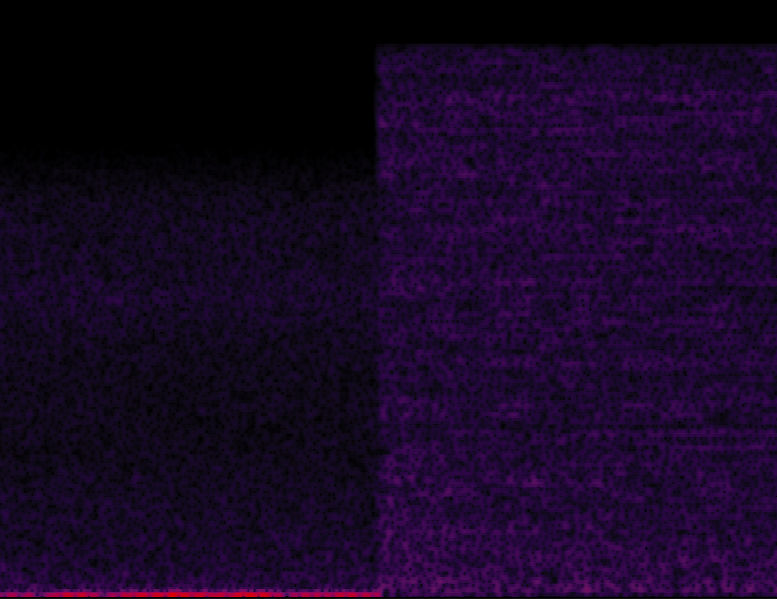
\includegraphics[width=.4\textwidth]{fourier.png}
	\caption{Porovnání šumové stopy projektu Rok 2025 (vlevo, využit \enquote{peřinový bunkr} pro snížení hladiny šumu) a~projektu Prosinec (vpravo).}\label{img:fourier}
\end{figure}
\subsection{Animování oblohy v~programu Stellárium}\label{makingof:stellarium}
Celý proces animování začíná prací se scénářem. Ze scénáře se vypíše seznam jednotlivých scén a~přechodů mezi nimi. Pro tento úkol jsem si vytvořil speciální formát zápisu, který obsahuje vše, co je potřebné k~vytvoření jednotlivých přechodů ve videu. Viz tabulka níže.

\begin{table}[h]
	\centering
	\begin{tabularx}{\linewidth}{lc*{5}{>{\RaggedRight\arraybackslash}X}}
	\toprule
	\# scény    & Směr scény & Čas          & Souhvězdí         & Speciální objekty      \\ \midrule
	0000        & Z obzor    & západ slunce & Labuť, Lyra, Orel & Letní trojúhelník      \\ \addlinespace
	0001        & SZ obzor   & západ slunce & dtto, Herkules    & Herkulův květináč, M13 \\ \addlinespace
	0002        & Z obzor    & západ slunce & dtto              & ---                    \\ \addlinespace
	\ldots      & \ldots     & \ldots       & \ldots            & \ldots                 \\ \bottomrule
	\end{tabularx}
	\caption{Demonstrace tabulky s~informacemi o~scénách}\label{tab:scenar}
\end{table}		

Většina animací, které se v~těchto videích nachází, byly vytvořeny pomocí simulačního programu Stellarium. Tento program je open-source (jeho zdrojový kód je volně dostupný) a~jeho primárním účelem je realistická simulace noční oblohy při pohledu očima nebo dalekohledem\fcite{stellarium:homepage}. Stellarium poskytuje širokou nabídku programovatelných rozhraní. Pro účely této práce využívám webový server, přes který lze instanci Stellaria ovládat z prohlížeče a~skriptovací rozhraní, které umožňuje interakci se Stellariem pomocí programovacího jazyka, založeného na standardu ECMAScript (využívaného například jazykem JavaScript\fcite{wiki:ecmascript}).

Největším problémem pro využití Stellaria v~produkci videí je fakt, že jeho tvůrci nepočítali s~jeho využitím pro tvorbu videí. Neexistuje tam například funkce, která by Stellariu řekla \enquote{Otoč se plynule na tyto souřadnice a~přitom nahraj video}. Jedinou možností, jak získat tuto animaci, je export každého samostatného snímku jako separátního souboru a~tyto jednotlivé snímky následně spojit do finálního videa pomocí nástroje jako FFmpeg. 

Prvním krokem v~tomto procesu je získání souřadnic jednotlivých snímků. Do tohoto momentu mám pouze informace o začátku a konci přechodu. Tyto informace obsahují azimut, výšku, přiblížení pohledu, datum a čas. Z těchto dat dále sestavím vektory $\vec{s}$ a~$\vec{e}$, které označují začátek a~konec přechodu v~pětidimenzionálním prostoru. 5D prostor je velice obtížné si představit, proto ho na~chvíli zjednodušíme do 2D prostoru. Zde jedna dimenze bude představovat azimut a~druhá výšku nad obzorem. 

\textcolor{red}{osy v demu}

Pro názornost tohoto konceptu tohoto konceptu jsem vyvinul nástroj, dostupný na \url{https://2ddemo.mp.itoncek.space}. V~levém horním rohu je zobrazena kartézská soustavu souřadnic, kde osa $x$ (znázorněná červeně) představuje azimut a~osa $y$ (znázorněná zeleně) představuje výšku nad horizontem. Umístění bílého křížku na grafu znázorňuje aktuální střed pohledu na obloze. Tím jsou definovány dvě dimenze z pěti.

Zbývající tři dimenze představuje přiblížení pohledu, čas a~datum simulace. V~tomto pětidimenzionálním prostoru se nachází každý snímek ze všech novějších videí AstroCrew. Každý snímek z obou projektů, které jsou tématem této práce, lze popsat pomocí souřadnic v~tomto prostoru.

Nyní máme matematicky definované počáteční a~koncové souřadnice snímků přechodů a můžeme využít rovnici lineární interpolace k~výpočtu souřadnic všech snímků, které leží mezi těmito limitními hranicemi.
\[c = (1-t)*a + t * b\] 
Tato rovnice převede každou hodnotu mezi $t=0$ (začátek přechodu) a~$t=1$ (konec přechodu) na hodnotu, která leží na úsečce $\overleftrightarrow{AB}$. Bod $A$ definujeme jako počáteční bod a~bod $B$ jako koncový bod přechodu. Tato rovnice se často nazývá \textit{lerp(a,b,t)} a~tuto definici budu po zbytek kapitoly používat. Poté pomocí lineární interpolace vypočítám vektory jednotlivých snímků v~přechodu.%chktex 36

\textcolor{red}{přejmenovat přechody v anim, přejmenovat quart na cub}

Výsledná animace je ve~výše zmíněném nástroji označena tlačítkem \enquote{Lineární přechod}. Animace je zde sice plynulá, ale začátky a~konce jsou trhané. Proto vstupní faktor $t$ nejdříve přetransformuji, abych se zbavil trhavých pohybů, které mohou být pro diváky nepříjemné. 

Je několik možností, jak tuto pomocnou transformaci provést. Jednou variantou je kvadratický přechod. Zde faktor $t$ upravíme pomocí rovnice:
\[u = lerp({t}^{2}, inv({inv}^{2}(t)), t)\]
Kde \textit{inv(x) = 1-x} a výsledný faktor $u$ použijeme dále ve standardní lineární interpolaci.  V~ukázce je tato animace označena tlačítkem \enquote{Kvadratický přechod}. Výsledný přechod začíná a~končí výrazně plynuleji, dosáhli jsme tedy toho, co jsme potřebovali. %chktex 36 %chktex 9 %chktex 15

Dalšími variantami jsou přechody kubický a exponenciální. Oba začínají sice plynuleji než kvadratický, ale ve střední části cesty naberou výrazně vyšší rychlost, která je v případě pozorování oblohy nepraktický a může být potenciálně nepříjemná pro diváky. Pro jiné aplikace může být naopak lepší volbou. Například se využívá v uživatelských rozhraních na mobilních telefonech, nebo dynamické zobrazení animovaných sloupcových grafů (například volebních preferencí nebo výsledků hlasování). Další nevýhodou kubického a~exponenciálního přechodu je relativní složitost vyjádření pomocí jedné funkce. Tyto přechody jsou často simulovány spojením dvou funkcí v~$t=\frac{1}{2}$. Obě dvě animace je možné najít ve výše zmíněném nástroji pod tlačítky \enquote{Kubický přechod} a~\enquote{Expo.\ přechod}.

Nyní máme trajektorii definovanou matematicky pomocí kvadratické funkce. Na trajektorii tedy můžeme rozmístit požadované množství snímků. Pro většinu animací v~našich videích používám 500 snímků, které tvoří 10 sekund finálního videa.

Nástroj StellariumPanoramaCreator, který jsem pro tento úkol vytvořil, výše popsanou matematiku implementuje do praxe. Ve skriptu je předem definováno, jaké kroky má Stellarium provést. Je volně dostupný na adrese \url{https://github.com/IToncek/StellariumPanoramaCreator}. Při svém běhu postupně prochází skrze předprogramované instrukce, které jsou zabudované přímo ve zdrojovém kódu a~generuje podle nich řádky skriptu a~případné složky, potřebné pro úspěšný běh skriptu. Mezi funkcemi, které často využívám se nachází například funkce \textit{setup()}. Připraví Stellarium pro zaznamenávání videa (vypne veškerá překrytí, změní model atmosféry, skryje objekty Sluneční soustavy, \ldots). Funkce \textit{move()}, která otočí kameru na pozici dodanou v~parametru \textit{orientation}, nastaví datum a~čas dodaný v~parametru \textit{datetime}. Další využívanou funkcí je \textit{cheese()}, která pořídí snímek v~aktuální orientaci a~uloží ho ve formátu TIFF.% chktex 36

Z těchto základních \enquote{stavebních} funkcí jsou poté sestavovány funkce komplexnějšího rázu, jako například funkce \textit{slideTo()}. Tato funkce vytváří primitivním způsobem skriptové soubory tak, že pro každý snímek definuje otočení pohledu, změnu času a~dne, změnu přiblížení a~uloží výsledný pohled do souboru. % chktex 36

Během přípravy této maturitní práce do sady funkcí přibyla nová kategorie funkcí, které nechávají veškeré výše uvedené výpočty na Stellariu. Tato nová metoda umožňuje využití automatického výpočtu trajektorie za běhu skriptu místo generování jednotlivých bodů trajektorie předem. 

Jednou z dalších nových funkcí je \textit{travelTrack()}, která vytvoří plynulý přechod mezi nebeskými souřadnicemi dvou objektů bez nutnosti zadávání jejich souřadnic do logiky skriptu. Další novou funkcí je \textit{slideTrack()}, která sleduje jeden vybraný objekt a~zajistí, že je na každém snímku přesně uprostřed. % chktex 36

Pro ukládání takto vygenerovaných snímků využívám formát TIFF, který mi poskytuje vysoce kvalitní data, komprimována bezztrátově pomocí algoritmu LZW.\@ Jeden takový snímek má rozlišení \(3840\times2160\) pixelů a~velikost 5--7MB.\@ Dohromady má jeden přechod mezi scénami velikost přibližně 7GB.\@ Pro celé video by to znamenalo velikost přes 200GB.\@ Aktuálně nevlastním žádný disk s~dostatečnou kapacitou a~rychlostí pro střih. Proto v~posledním kroku příprav převedu každý přechod do formátu ProRes, který mi umožňuje snížit velikost na pouhých 10GB, za cenu minimální ztráty na kvalitě. 

Při kompilaci jednotlivých snímků do videí nastavuji finální snímkovací frekvenci projektu, jíž je pro AstroCrew 50 sn./s. Tato snímkovací frekvence je v~souladu s frekvencí evropské elektrické sítě, standardy Evropské unie a~příjemná pro oko diváka.

Pro video o~\enquote{Úkazech na obloze v~roce 2025} jsem zvolil trochu jiný postup. Přechody ukládám ve formátu JPEG2000, který používá ztrátovou kompresi. Celé video je tak možné na konci procesu vyrendrovat znova a~opravit případné drobné detaily, které ve videu mohly vziknout v~průběhu jeho tvorby.\fcite{jpeg2000}
\subsection{Kompletace videa v~programu DaVinci Resolve}\label{makingof:resolve}
\subsubsection{Struktura videa}\label{makingof:resolve:structure}
Každé video se skládá z mluveného slova, hudby, simulace noční oblohy, scénáře a titulků. Základem celého videa je mluvené slovo, kterému se přizpůsobují všechny další složky. Mluvené slovo vložím na časovou osu a rozdělím na jednotlivé odstavce tak, aby mezery byly v momentech, kdy bude potřebný přechod v simulaci oblohy. Poté začnu na časovou osu rovnat jednotlivé obrazové části.

V úvodu videa diváky přivítáme a stručně jim představíme obsah dílu. Zároveň je upozorníme, že informace uvedené ve videu neplatí po celém světě, ale pouze kolem 50.\@ rovnoběžky severní šířky a pouze v uvedeném časovém rozmezí. Zde také shrneme krátce podmínky pro pozorování noční oblohy v daném měsíci. V této části obrazová stopa ukazuje časosběry s astronomickou tématikou, nejčastěji pohledy na noční oblohu nebo výhledy z Mezinárodní vesmírné stanice. Tato videa nevznikají ze simulací ale jedná se o videa všeobecně dostupná.

V hlavní části videa využíváme jako podklad mluveného slova simulace ze Stellaria, které jsme získali postupem popsaným výše. V této části jsou na obloze zobrazeny jednotlivé hvězdy, jejich spojnice, které vytvářejí tvary souhvězdí, a umělecké ztvárnění souhvězdí, korespondující s jejich názvy. Takto divák může lépe souhvězdí nalézt, když se podívá na skutečnou noční oblohu. 

Během představování každého souhvězdí jsou popisovány i zajímavé objekty hlubokého vesmíru, které lze v oblasti daného souhvězdí nalézt. Mezi snadno viditelné objekty hlubokého vesmíru se řadí hvězdokupy, mlhoviny a galaxie. Existují i další objekty hlubokého vesmíru, jako například černé díry nebo aktivní galaktická jádra, která ale nemůžeme snadno pozorovat bez speciálního vybavení (např.\ zrcadlový dalekohled GTC na Kanárských ostrovech, dalekohled VLT --- Very Large Telescope na poušti Atacama v Chile nebo Hubblův vesmírný teleskop), a z tohoto důvodu je v našich videích neuvádíme.

Souhvězdí a~objekty hlubokého vesmíru jsou ve videu chronologicky řazeny podle nejlepšího času pozorování v průběhu noci --- od západu k~východu slunce. 

V následující části zmiňujeme nejdůležitější astronomické události, které v průběhu měsíce pravidelně nastávají. Jedná se například o meteorické roje, noční svítící oblaka a pravidelné charakteristiky podmínek pozorování (např.\ v zimě jsou na pozorování nejlepší podmínky, ale je chladno a doporučujeme proto divákům s tím počítat, nežli vyrazí do mrazivé noci nepřipraveni). Tento koncept videa umožňuje jej pravidelně používat každý rok v daném měsící bez nutnosti jakýchkoliv úprav.

\subsubsection{Časová osa scény}\label{makingof:resolve:merging}
Následující obrázek zachycuje uspořádání jednotlivých částí scény na časové ose.

\begin{figure}[H]
	\centering
	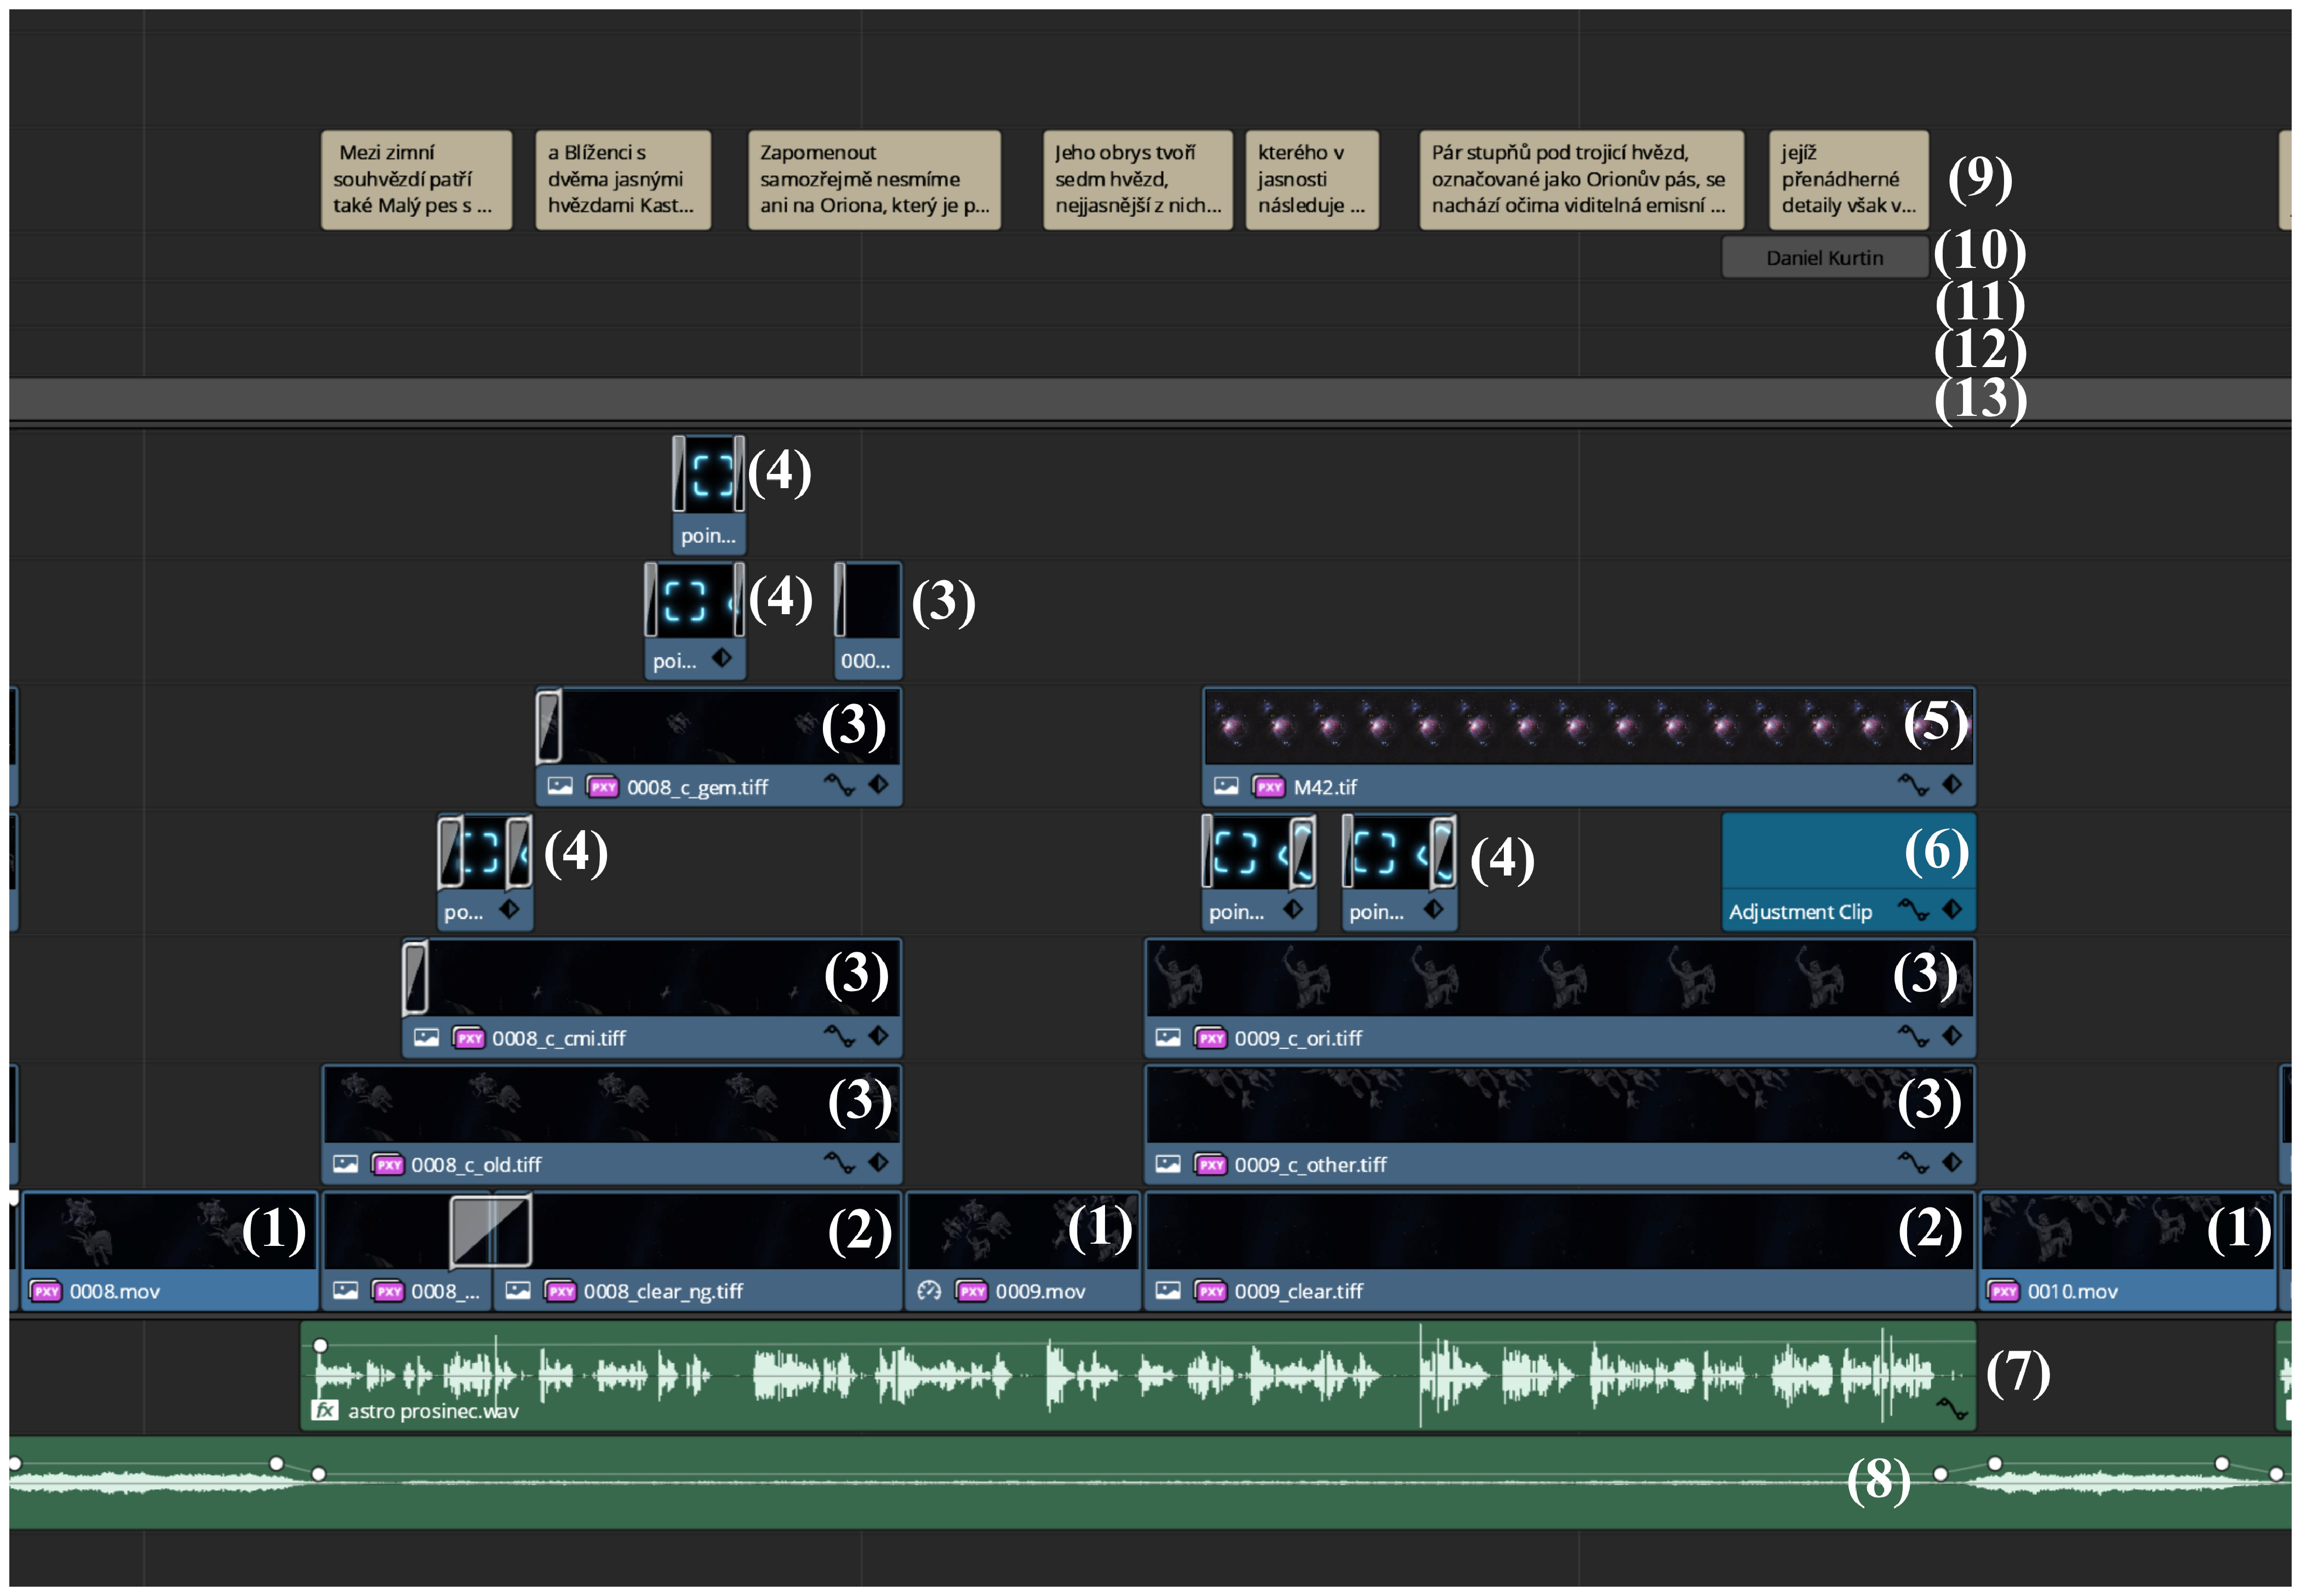
\includegraphics[width=1\textwidth]{timeline_annotated.eps}
	\caption{Časová osa jedné ze scén. Každá důležitá část scény má přiřazené číslo.}\label{img:timeline}
\end{figure}
Číslo 1 označuje animace, při kterých se obraz pohybuje, a až na vyjímky neobsahuje mluvený komentář. Animace slouží k posunu pohledu pozorovatele do jiné části oblohy, čímž pozorovatel neztratí orientaci na obloze. 

Číslem 2 je označen statický snímek, který slouží jako podklad pro danou scénu. Číslo 3 označuje snímky jednotlivých souhvězdí. Oba tyto typy snímků vznikají samostatně zároveň s generováním předchozí animace v programu Stellarium.

Číslo 4 označuje tzv.\ pointer. Jedná se o animovaný klip zářícího výrazného pulzujícího čtverce se zaoblenými rohy. Tím je zvýrazněn objekt o~kterém právě pojednává scénář. Pointer je zobrazen na obrázku~\ref{img:pointer}. 

\begin{figure}[H]
	\centering
	
\includegraphics[width=.5\textwidth]{pointer.eps}
	\caption{Pointer --- animace využívaná pro upřesnění pozice objektu, o~kterém v~daném momentě hovoří.}\label{img:pointer}
\end{figure}

Číslo 5 označuje snímky objektů hlubokého vesmíru, které jsou do snímku uvedeny nejdříve pomalu na místě, kde se objekt na obloze nachází. Jakmile se komentář zmíní o daném objektu, spustí se animace, která obrázek zvětší, dá divákovi několik sekund na prohlédnutí obrázku, a poté obrázek zase stejným způsobem zmizí.

Číslem 6 jsou označeny tzv. Adjustment Clips. Těmito klipy mohu ovlivnit všechny části scény, které se nachází na časové ose pod nimi. V případě situace ukázané na obrázku~\ref{img:timeline} se jedná o ztmavení všech nižších vrstev, aby lépe vynikla fotografie Velké mlhoviny v Orionu, kterou pořídil náš scénárista Daniel Kurtin.

Číslem 7 je označena stopa s mluveným slovem a číslem 8 je označena hudební stopa. Obě stopy běží většinou souběžně. V místech mluveného komentáře je hlasitost hudební stopy potlačena, aby bylo mluvené slovo zřetelně slyšet.

Čísla 9 --- 13 označují titulkové stopy. Jejich počet a využití se mění podle požadavků daného projektu. Tyto stopy využíváme nejen pro standardní využití ve formě titulků v~češtině a~někdy v~angličtině, ale využíváme je i~jako prostor pro citování zdrojů obrazových materiálů, pro opravu chyb v~již vydaném videu, pro poznámky a~doplnění obsahu od editora a~pro stopu s~informacemi o~zdrojích hudby. Tento přístup využíváme zejména kvůli jednoduchosti tvorby titulků, možnosti jejich úpravy po vydání videa a~možnosti je skrýt, pokud jimi nechci být rušen. 
\subsubsection{Mixování obrazové části}
Další úpravy obrazové části jsou zaměřeny na vrstvení jednotlivých částí scény přes sebe. Bez těchto úprav není možné skrz jednotlivé vrstvy vidět, co je pod nimi. Například by bylo vidět pouze jedno souhvězdí nebo objekty hlubokého vesmíru by byly na černém pozadí místo jejich prolínání s atmosférou.

Záběry jsou vrstveny přes sebe pomocí metody Lighten přímo v programu \textcolor{red}{zkontrolovat velká písmena} Davinci Resolve, která pro každý pixel obrázku vybere nejjasnější barvu ze všech vrstev na daném snímku videa. Toto umožňuje vzájemné překrytí obrázků souhvězdí a objektů hlubokého vesmíru, aniž by bylo třeba odstraňovat u~každého pozadí. 

Úprava pro objekty hlubokého vesmíru probíhá následovně:

Nejprve získám obrázek daného objektu z internetu, například z Wikipedie, která poskytuje jasné licenční podmínky. Pokud na Wikipedii není vhodný nebo dostatečně kvalitní obrázek, prohledám další fotografie na internetu. Občas ani tento krok nestačí, zejména u~objektů nezajímavých na focení. Poté využiji celooblohové sady dat, například Digitized Sky Survey 2 nebo Mellinger color optical survey, které lze získat z Centra astronomických dat univerzity ve Štrasburku díky jejich nástroji Aladin. Tyto sady dat pokrývají značnou část celé oblohy a~v České republice pokrývají 100\% viditelné oblohy. 

Získané fotografie následně upravuji pomocí software Zoner Photo Studio X, kde upravím kontrast pozadí tak, aby bylo absolutně černé a~tudíž při kompletaci zmizelo. Následně odstraním hvězdy blízko okraje snímku, aby byl přechod mezi snímkem a~pozadím méně znatelný. Takto pracuji pouze s obrázky z jiných zdrojů než ze Stellaria.
\subsection{Mixování zvukové části}
Ve zvukové části jsou na sebe vrstvy stopy hudby a~mluveného slova. Hudbu vybírám ze seznamu hudby v~knihovně YouTube a~ze seznamu skladeb, využívaných softwarem SpaceEngine. SpaceEngine je simulátor vesmíru, zaměřen spíše na jiné pohledy na vesmír než ze Země. Jeho hudební knihovna obsahuje skladby které mají evokovat atmosféru různých míst ve vesmíru. Při vybírání hudby k videu je základním kritériem, aby hudba diváka nijak nerušila a zároveň dotvářela atmosféru celého videa. Jako úvodní hudbu v~našich videích používáme skladbu \textit{Beyond --- Patrick Patrikios} ze zvukové knihovny YouTube. V~hlavní části se objevují skladby z software SpaceEngine, jako například \textit{Space G Lydian --- Alfred Potter}, \textit{The Blithering Heights --- Akira} a~\textit{A peaceful Place --- Goodstreet}. V závěru videa využíváme skladbu \textit{Instant Crush --- Corbyn Kites} znovu ze zvukové knihovny YouTube.
\section{Historie popularizace astronomie}
Astronomie se začala rozvíjet, stejně jako většina ostatních věd, již ve starověku. V různých kulturách byla využívána k různým účelům. \textcolor{red}{egyptská hustá věc, náboženství} \fcite{arxiv:egypt}. Mořeplavci používali od pradávna pozice hvězd k navigaci na moři, například pomocí sextantu. \textcolor{red}{rejpnout si do astrologie}. \textcolor{red}{aristotelovy myšlenky, ptolemaios, země kulatá}.

Ve středověku byly tyto vědomosti znepřístupněny náboženstvím a náboženskými dogmaty. \textcolor{red}{koperník, galileo, brahe?, kepler, newton, hvězdárny}

K výraznému rozvoji došlo až během vědecko-technické revoluce s dostupností optiky a elektroniky a znovu pak s začátkem letů do vesmíru. Knihy, časopisy, fotografie, filmy, rádio, televize, planetária robo.

Dalším velkým skokem byl vzestup počítačů a internetu. Vznik planetárií digi + 3D, vzdělávací videa a přenosy.
\section{Historie a~vývoj procesu tvorby astronomických videí}
Proces tvorby našich astronomických videí se v~průběhu let výrazně měnil a vyvíjel. První video jsme vytvořili v~roce 2021 a~od té doby jich vzniklo dalších 10.V této části se podíváme na celou historii tvorby astronomických videí skupinou AstroCrew.
\subsection{Začátky --- Prosinec 2021}
Naše cesta začala 14.\ prosince 2021, kdy jsme vydali naše první video. Toto video nebylo primárně určeno k~vydání na platformě YouTube, ale bylo vytvořeno pro planetárium v~iQLandii, kde jsme ho představili již 9.\ prosince 2021 na pravidelné akci \enquote{Večery pod hvězdami}. 

Celé video je vytvořeno pro promítání v planetáriu a z tohoto důvodu je promítnuto sféricky, jak můžete vidět na obrázku~\ref{img:prosinec}. Pro vydání na YouTube jsme toto video modifikovali, aby ho YouTube akceptoval jako 360° video, i~když polovina videa je čistě černá (vše co je pod horizontem planetária není vidět). 

Produkce tohoto videa byla velice náročná. V~té době jsem pro střih využíval stříhací program Adobe Premiere Pro. Software byl velice nestabilní, zvláště s náročností 4K videa a složitými transformacemi na sféru. Veškerá tvorba animací tehdy probíhala výhradně manuálně a byla tedy časově náročná. 

Toto video jsem natáčel tak, že jsem namířil Stellarium podobně, jako je namířená kopule planetária v~iQLandii a~poté jsem pomocí přesouvání času přemisťoval souhvězdí a~jednotlivé objekty tak, aby byly co nejlépe vidět. 

Následně jsem pomocí programu Adobe After Effects vložil do scény obrázky daných objektů hlubokého vesmíru pomocí integrovaného efektu VR Converter. Díky technologii Adobe Dynamic Link jsem poté jen vložil kompozice z After Effects přímo do časové osy v~Premiere Pro a~nemusel jsem je exportovat. 

Bohužel tento přístup je neskutečně pomalý a~snižuje významně výkonnost celého stříhacího programu. Z tohoto důvodu je Prosinec 2021 jediným videem vytvořeným v~tomto stylu.

\begin{figure}[ht]
	\centering
	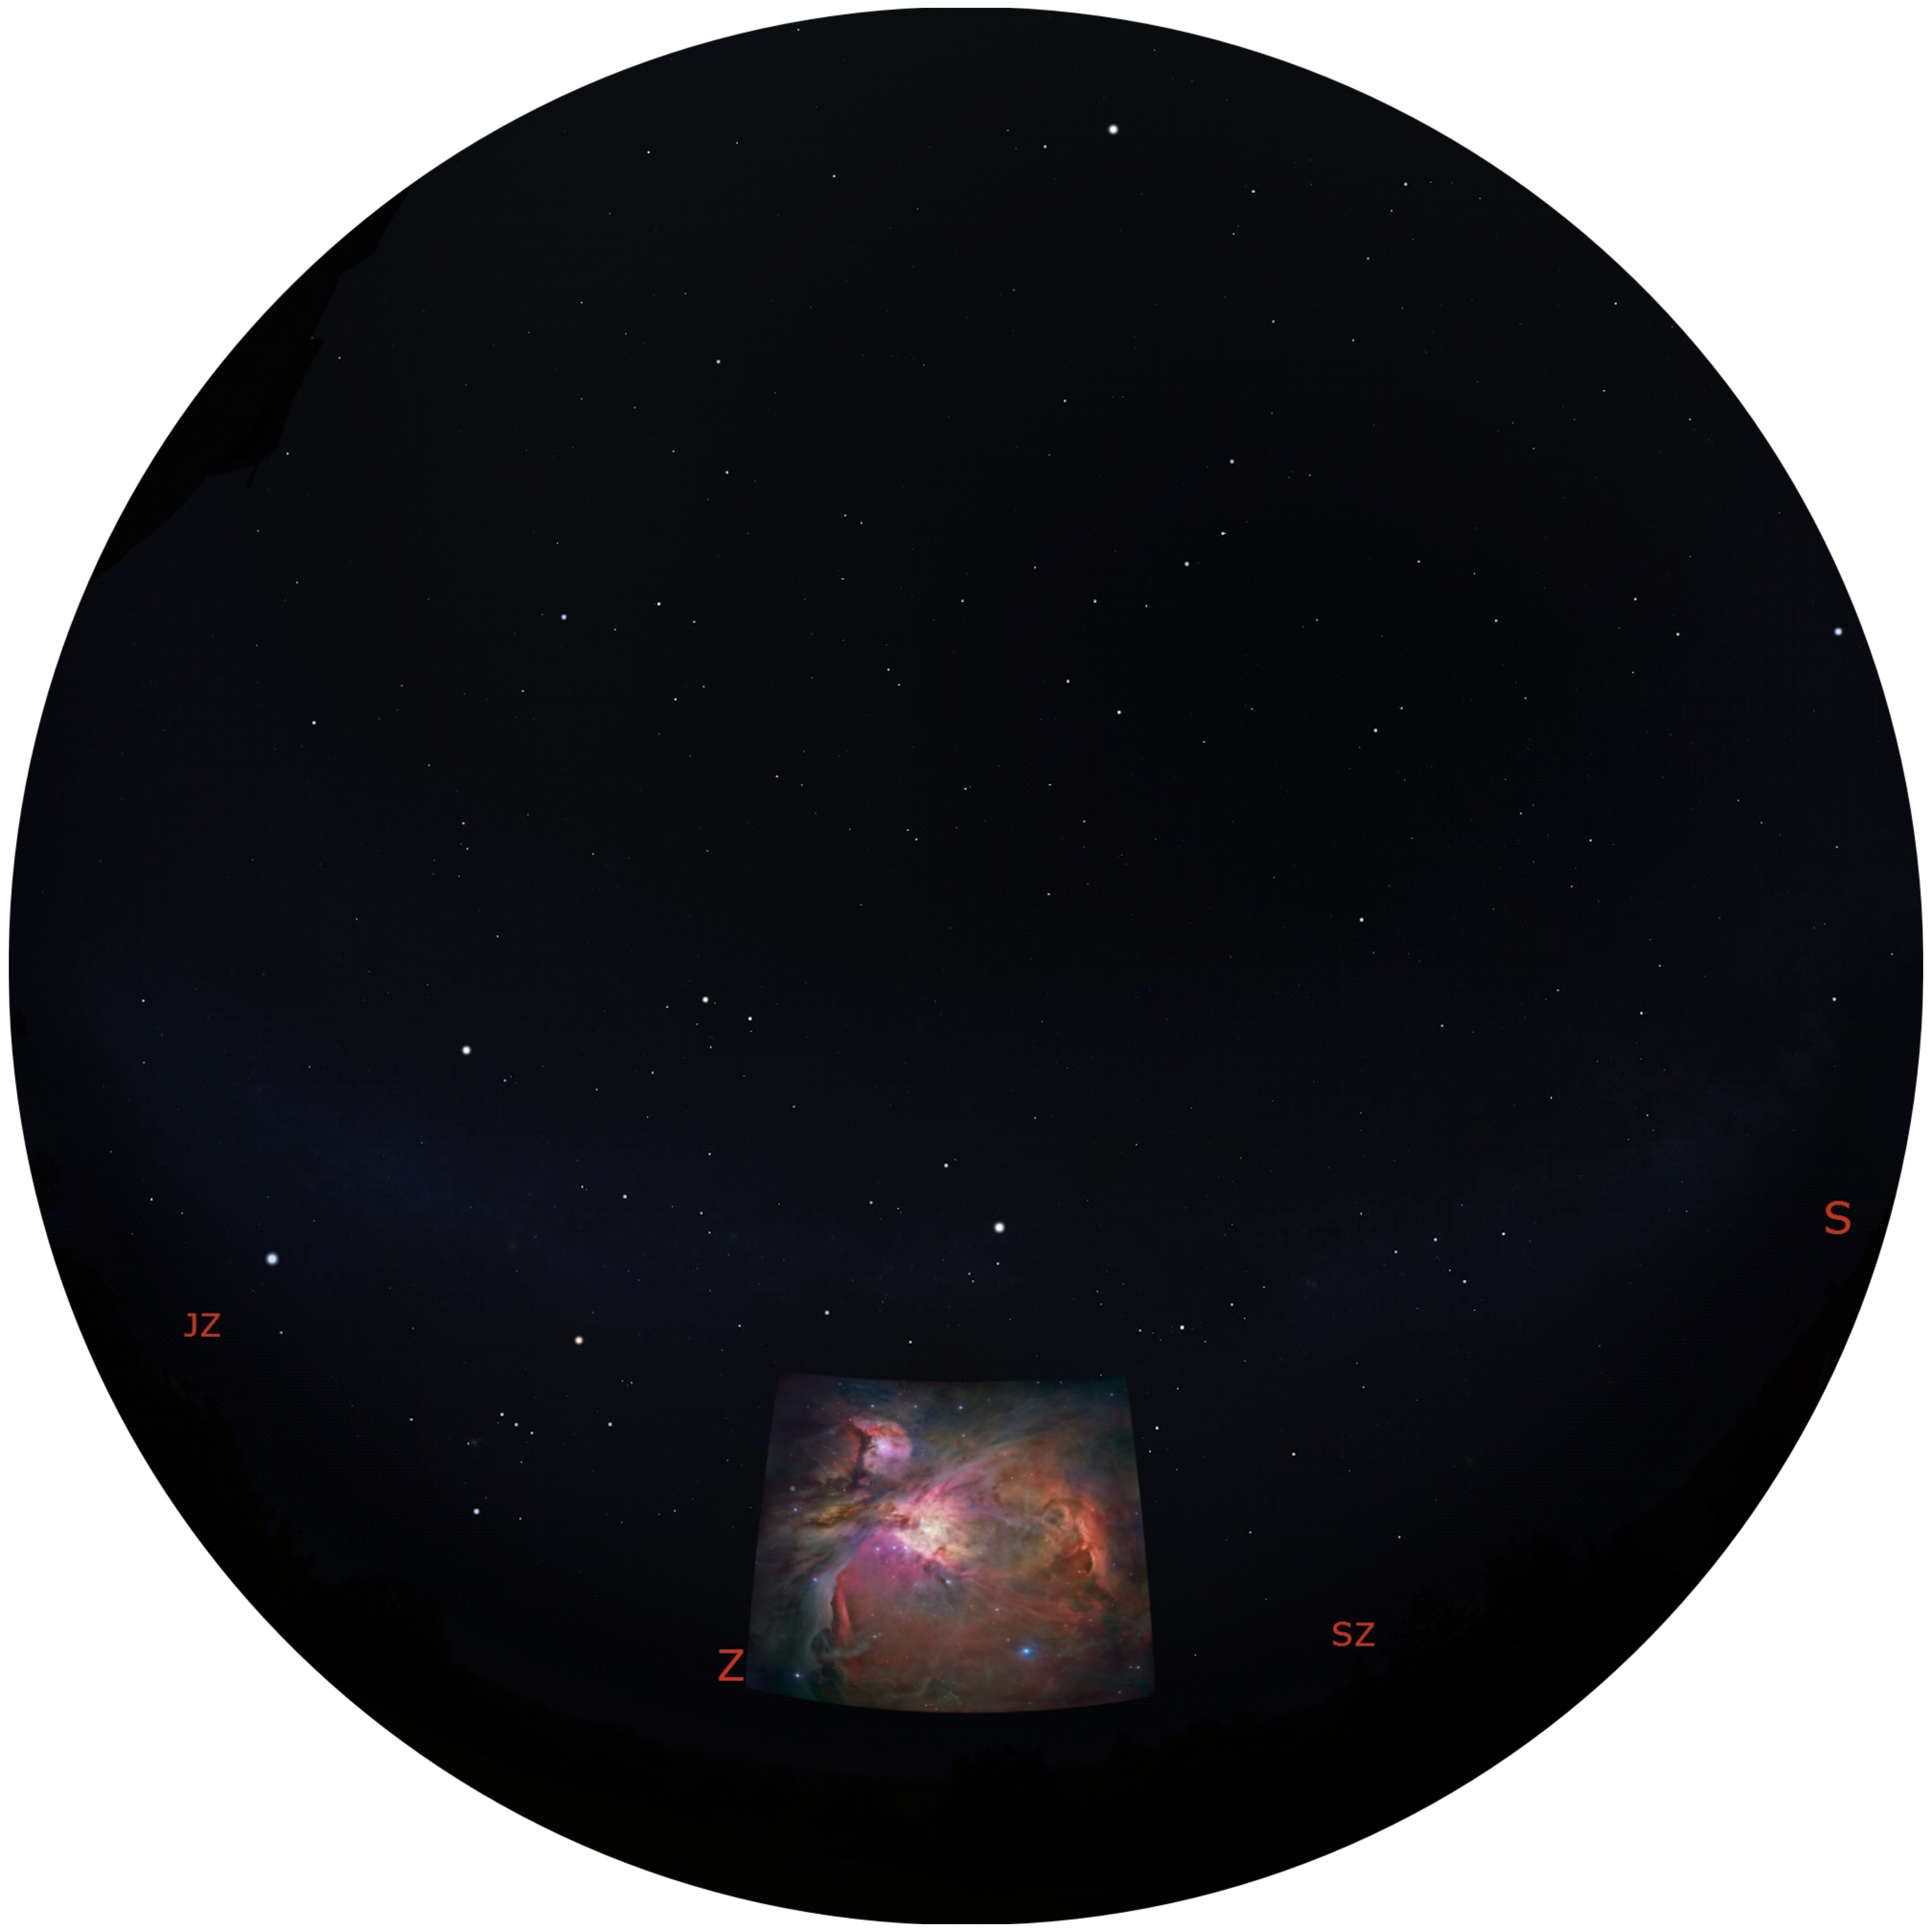
\includegraphics[width=.7\textwidth]{prosinec.eps}
	\caption{Demonstrace našeho prvního videa.}\label{img:prosinec}
\end{figure}
\subsection{Jednoduchá éra --- Březen až Květen 2022}
Celý proces, jak jsem ho popsal v~sekci~\ref{makingof} je aktuálním stavem tvorby. Na úplném začátku produkce tento proces ještě neexistoval a~veškeré znalosti potřebné pro tvorbu \textquote{moderních} videí bylo nutné získat postupným experimentováním. Videa v~této éře byla velice jednoduchá. Animace byly vytvořeny nahráváním okna Stellaria a~jeho ovládáním přes webové rozhraní.

Ačkoliv tento proces byl jednoduchý na provedení, byl náročný na čas. Pokud jsem netrefil objekt, bylo nutné se vrátit na předchozí a~nahrát celý přechod znovu. Když se Stellarium zaseklo někde během přechodu, bylo nutné daný přechod nahrát znovu. Tyto situace se mohou zdát banální, ale při množství přechodů, které byly v~té době ve videích, se tyto časové nároky nasčítaly a~výrazně zpomalily celou produkci videa. Ukázka finálního videa z této éry je připojena níže jako obrázek~\ref{img:brezen}.

\begin{figure}[ht]
	\centering
	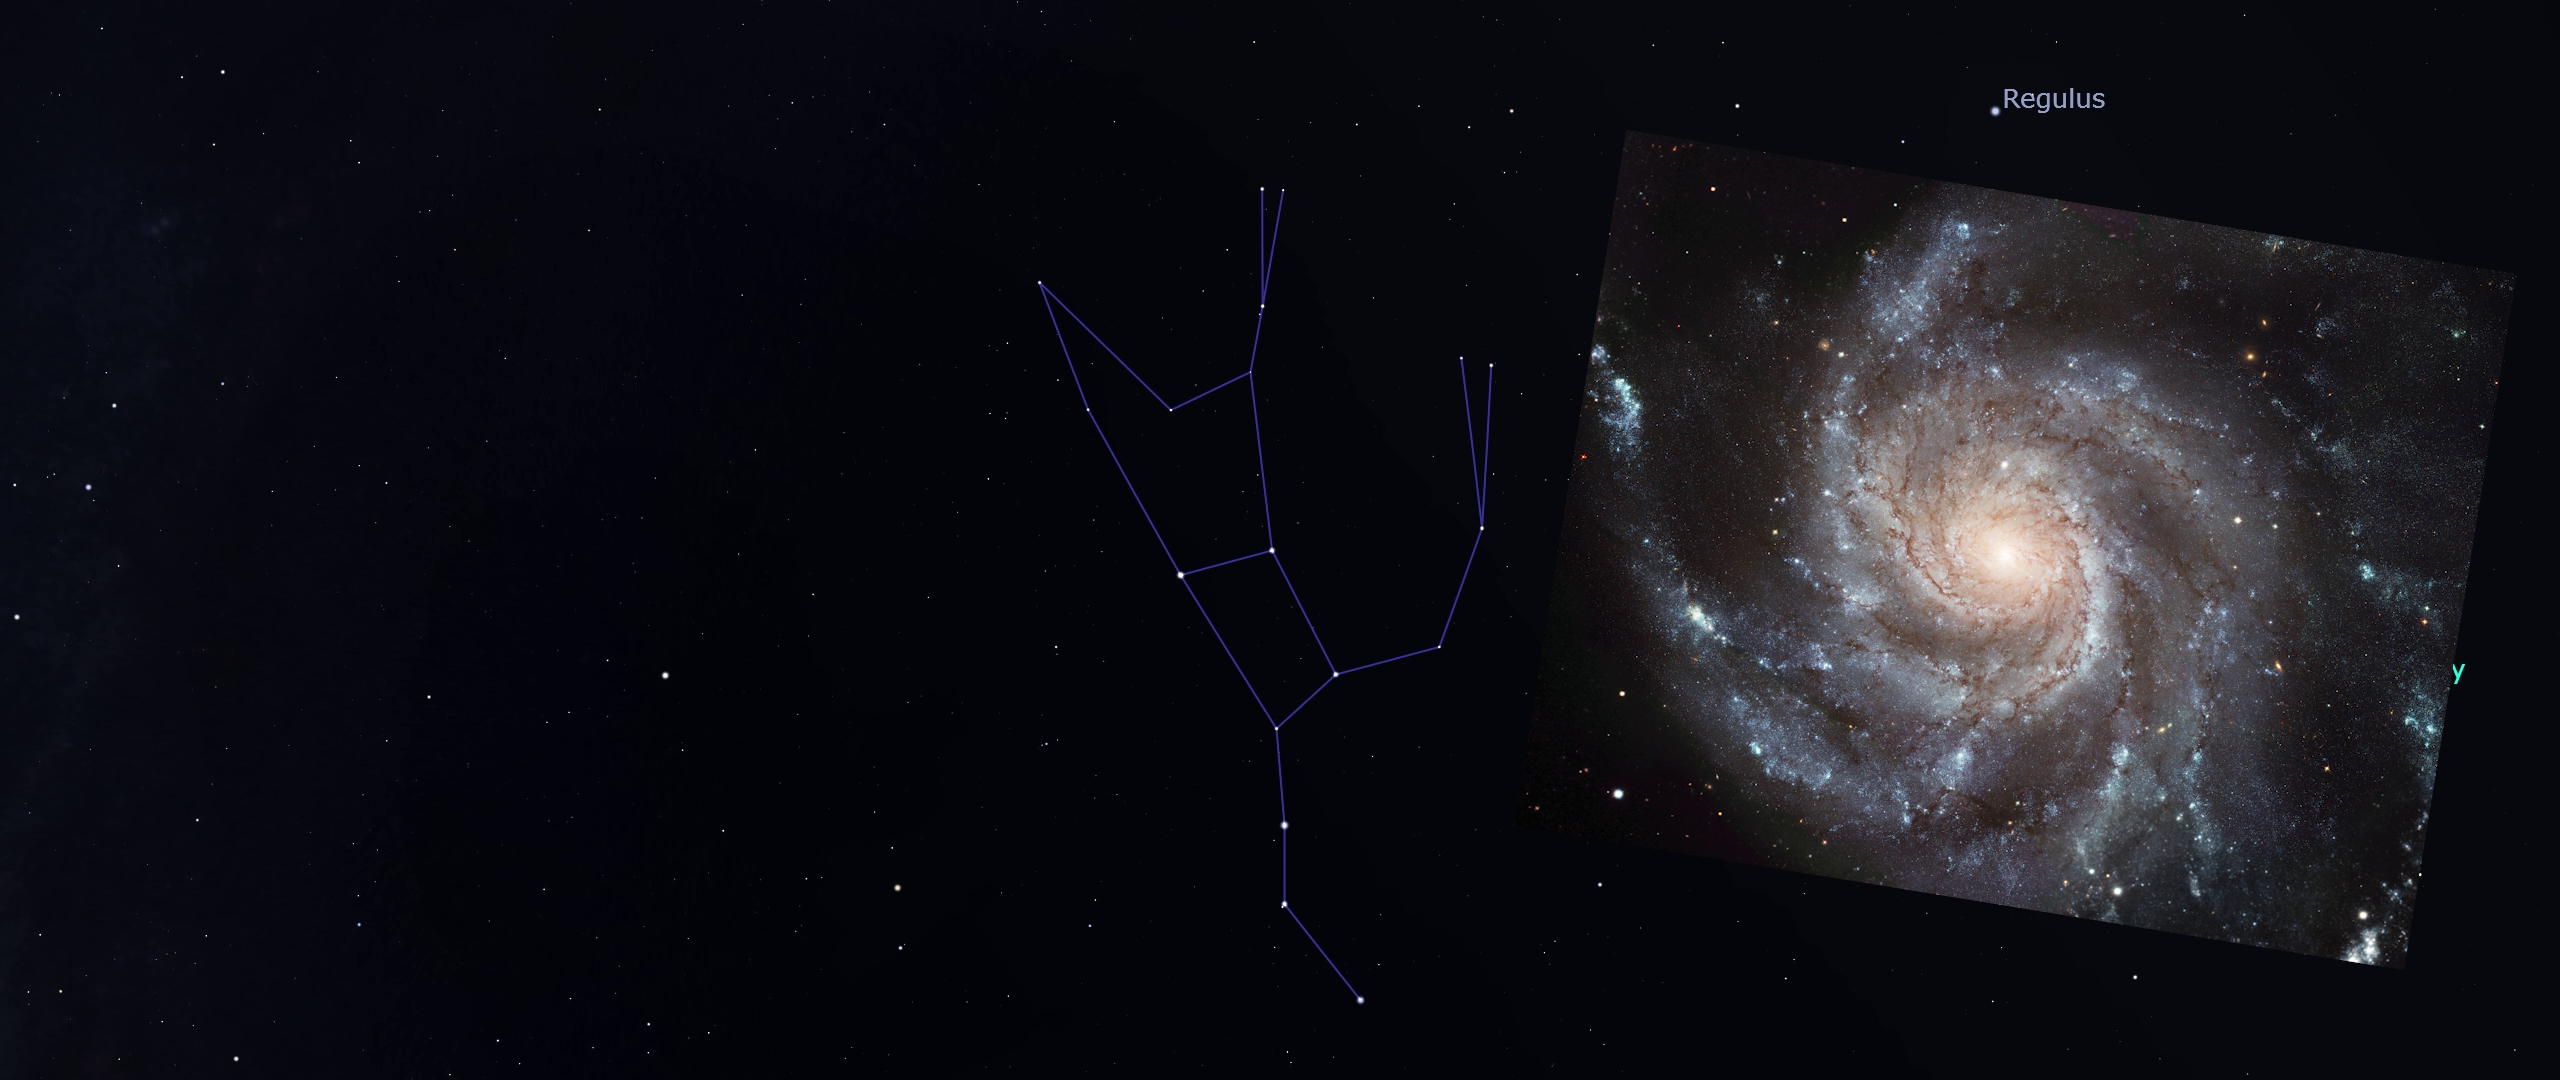
\includegraphics[width=.85\textwidth]{brezen.png}
	\caption{Demonstrace našeho prvního videa.}\label{img:brezen}
\end{figure}

Do této éry patří ještě video s~názvem \textquote{Jak pozorovat zatmění Měsíce 16.5.2022}, které vybočuje svojí tématikou. Vydali jsme ho 13. 5. 2022 jako návod na pozorování nadcházejícího zatmění Měsíce. Toto video značí přechod k~další éře, protože neobsahuje ani jeden záběr ze Stellaria. Skládá se primárně ze záběrů zatmění měsíce a~animace vygenerované pomocí systému Space Engine. Ačkoliv toto video má největší počet shlédnutí na našem YouTube kanálu, má relativně nízký dopad na náš YouTube kanál, protože většina těchto shlédnutí je ze stránek astro.cz a~seznamzpravy.cz, kam toto video nasdílel Martin Gembec, vedoucí planetária v~iQLandii.
\subsection{Éra spěchu --- Červen a~Červenec 2022}
Červnové a~červencové Astronomické desetiminutovky byly stříhány ve velikém spěchu. S~příchodem prázdnin se množství volného času, který jsem měl k~dispozici na stříhání se snížilo, a~tudíž bylo třeba produkci optimalizovat. V~této době jsem také začal přecházet do nového stříhacího programu, zvaného DaVinci Resolve, který využívám doteď. Tato změna prostředí produkce znamenala, že videa musela být jednodušší na produkci a~tudíž kvalita lehce upadla. Ukázku finálního videa jsem připojil v~přílohách jako obrázek~\ref{img:cervenec}.

\begin{figure}[ht]
	\centering
	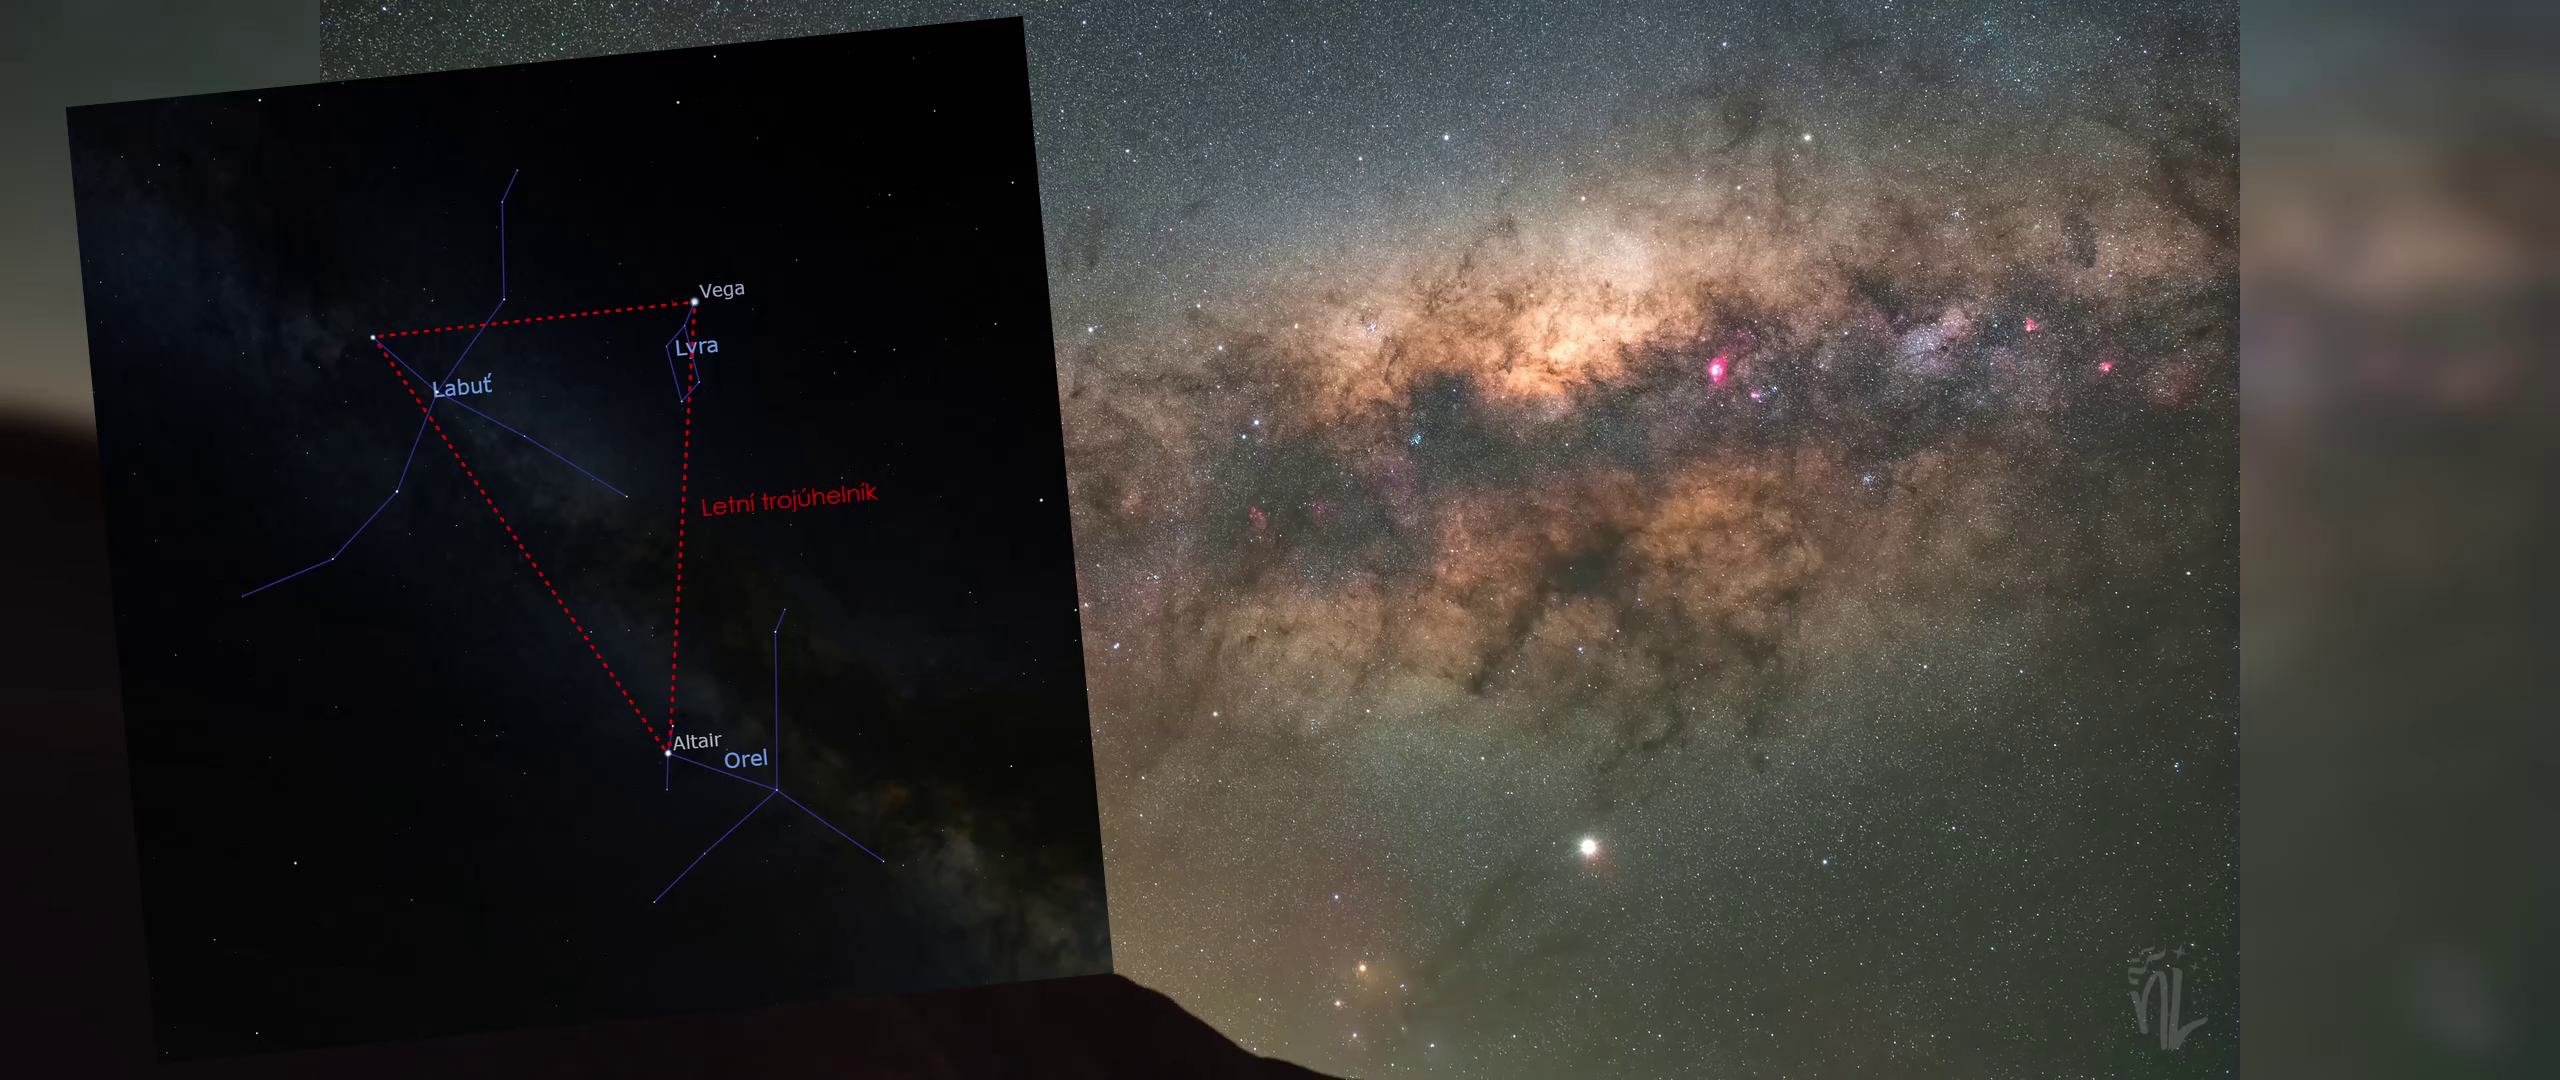
\includegraphics[width=.85\textwidth]{cervenec.png}
	\caption{Demonstrace Červencového videa.}\label{img:cervenec}
\end{figure}

Tato videa jsou jednoduchá, složená z časosběrných záběrů se zvukovým komentářem a~občasnými grafikami, vytvořenými ručně ve Stellariu. Videa jsou opravdu základní. Rád se bych je v~budoucnu pokusil se je předělat na moderní formát. Nicméně tato éra sloužila jako další nezbytný krok k~modernímu procesu, který se poprvé projevil v~únorových Astronomických desetiminutovkách.
\subsection{Renezance Astrocrew --- Únor 2023}
Únorové video je první, které se dá kategorizovat do skupiny moderních AstroCrew videí. V~této době jsem poprvé začal pracovat se Stellariem jako s~nástrojem pro generování snímků, která jsou později spojovány do videa. Zbavil jsem se tak přímého nahrávání videa, které předtím zabralo výraznou část času produkce.

Základní nápad této metodiky byl jednoduchý: nafotit celooblohovou panorámu, složit jí do jednoho snímku a~ten poté otáčet ve stříhacím programu. V~této době jsem začal tvořit nástroj StellariumPanoramaCreator (dále jen SPC), který se již v~produkci udržel. První verze SPC byla velice jednoduchá. Skript převzal kontrolu nad klávesnicí a~myší mého počítače a~pomocí integrovaného okna přímo ve Stellariu, které umožňovalo zadat azimut a~výšku, postupně nafotilo všech 54 snímků. Z nich se složila finální panoráma za pomoci programu Hugin, který obdržel všechny snímky a~projektový soubor s informacemi o pozicích snímků vygenerováný při běhu SPC.\@

Zpracování těchto dat bylo mnohem komfortnější než skládání videí natočených manuálně. Proces stále vyžadoval mnoho práce, než byla získána vstupní data. Tento čas nebylo možno nijak jinak využít, protože při běhu SPC nebylo možné využívat klávesnici ani myš. Nebylo možné ani odkliknout z okna jinam, protože v ten moment SPC ovládá klávesnici a myš. Mohl jsem pouze sedět a sledovat, co se děje na obrazovce. Snímání jedné panorámy trvalo 10 --- 15 minut. Proto dalším logickým krokem bylo převedení komunikace SPC se Stellariem za oponu. 

Ideálním řešením se ukázalo webové rozhraní Stellaria. Tento modul je určen pro řízení Stellaria z tabletu nebo jiného počítače v~případě, že není možné ovládat přímo počítač se Stellariem, například pokud je počítač využíván pro demonstraci na hvězdárně. Na pozadí tento systém využívá protokol HTTP, který umožňuje přistupovat k~specifickým částem kódu Stellaria přes síť. Tento modul byl vznikl jako projekt v~rámci akce \textquote{ESA Summer of Code 2015}\fcite{stellarium:rcDoc}. 

Dokumentace\fcite{stellarium:rcAPI} tohoto protokolu je bohužel v~některých místech relativně chaotická a~nečitelná. Pro vývoj jsem tedy použil existující HTML rozhraní. Pomocí vývojářských nástrojů, dostupných ve většině moderních prohlížečů, jsem postupně zjistil veškeré adresy a~parametry, které Stellarium potřebuje. Poté jsem nástroj SPC přepsal, aby místo ovládání klávesnice a~myši využíval nově dostupné HTTP dotazy. Po náročné optimalizaci načasování jednotlivých příkazů se časová náročnost snížila přibližně na polovinu předchozího času a~celý proces mohl nyní proběhnout na pozadí. Ukázku finálního videa je na obrázku~\ref{img:unor}.

\begin{figure}[ht]
	\centering
	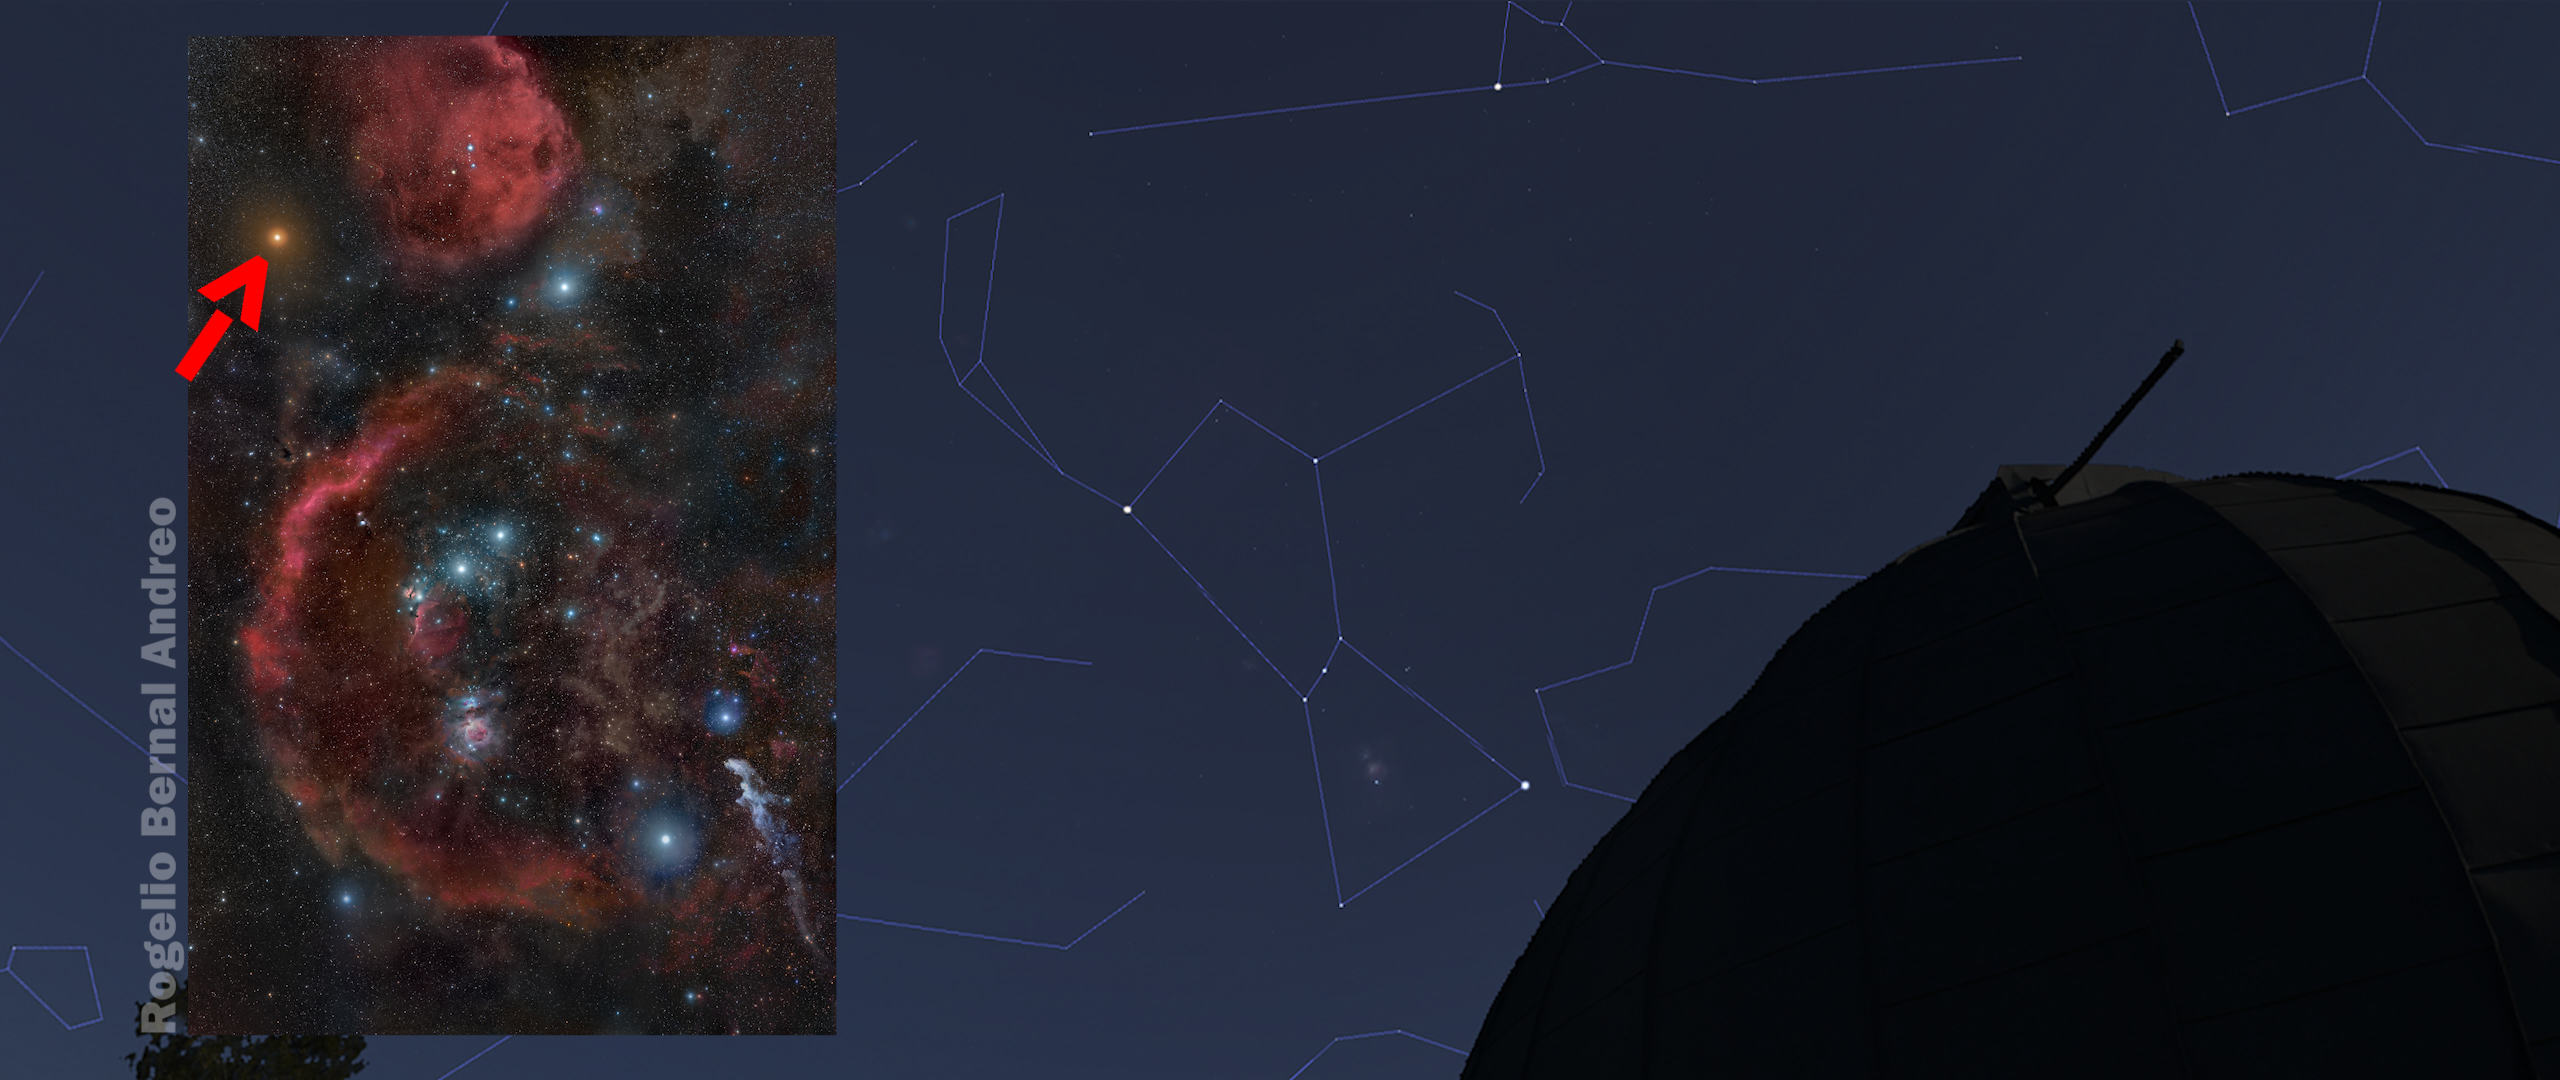
\includegraphics[width=.85\textwidth]{unor.png}
	\caption{Ukázka videa z února 2023.}\label{img:unor}
\end{figure}

V této fázi střih probíhal zpět v~Adobe Premiere Pro primárně kvůli pluginu Gopro FX Reframe. Ten panorámu vygenerovanou v SPC převedl na perspektivní zobrazení. Tento systém měl mnoho výhod oproti předchozímu procesu, při kterém bylo nutné perfektně trefit načasování při natáčení. Když se něco nepodařilo, bylo nutné celý segment natočit znovu. V~této nové verzi procesu stačilo při nějaké chybě přeanimovat poslední přechod a~upravit časování sekvence. I~tak, tento postup nesl značné nevýhody. Hlavní z nich byla vysoká zátěž počítače, z části způsobená náročností samotného stříhacího programu. Tento fakt znamenal, že render Únorových Astronomických desetiminutovek zabral 90 minut na výsledných 12 minut videa. V~říjnu 2023 se navíc plugin Gopro FX Reframe úplně přestal fungovat, což zrušilo vydání říjnových Astronomických desetiminutovek. Proto pro následující projekt bylo nutné vyvinout nový proces. 
\subsection{Moderní Astrocrew --- videa Rok 2024, Prosinec 2024 a~Rok 2025}
V listopadu roku 2023 přinesl Dan do naší skupiny nápad vytvořit video shrnující úkazy, které budou vidět v~roce 2024 na obloze. Po nedávném neúspěchu ve tvorbě říjnových Astronomických desetiminutovek bylo nutné změnit celý proces. Prvním pokusem bylo využití animačního programu Blender a~zachování exportu panorám a~jejich pozdější přemapování do perspektivního zobrazení. 

Tento postup sice fungoval, ale při tvorbě jsem byl nucen každé video exportovat \(2\times \), jednou jako panorámu a~jednou jako animovaný přechod. Během pokusů s~touto metodou mě napadla revoluční myšlenka. Místo exportu celé panorámy, ze které jsem pokaždé minimálně polovinu zahodil, exportovat pouze potřebnou oblast pro finální video. 

V této epoše se StellariumPanoramaCreator (dále jen SPC) jsem již přepsal téměř do současné podoby. Jako vstupy sloužily souřadnice a~časy jednotlivých přechodů. SPC následně ovládal Stellarium pomocí HTTP, jako v~předchozí éře. Výstupem bylo 500 snímků pro každý přechod v~rozlišení \(3840\times2160\) pro složení do finálního videa. 

Ačkoliv tento postup byl výrazně rychlejší a~příjemnější, odhalil jsem také několik slabých stránek implementace webového rozhraní Stellaria. Stellarium je schopné z webu zpracovávat příkazy pouze sekvenčně, tudíž není možné odeslat všechny příkazy naráz a~jen počkat, než se Stellarium vzpamatuje. Místo toho je nutné načasovat každý příkaz tak, aby strávil ve frontě příkazů minimum času. 

Tímto způsobem bylo vytvořeno video \textquote{Co nás čeká na obloze v~roce 2024?}. Pro videa \textquote{Astronomické desetiminutovky --- Prosinec} a~\textquote{Co nás čeká na obloze v~roce 2025?} byla provedena malá změna. Příkazy se přestaly odesílat přes HTTP, ale byly zapsány přímo do skriptového souboru Stellaria, které následně tyto příkazy spustilo v~maximální dostupné rychlosti. To umožnilo dosáhnout minimálních časových ztrát při běhu skriptu a zajistilo maximální efektivitu.
\newpage
\part{Praktická část}
\section{Astronomické desetiminutovky --- Prosinec}
Prosincové video je druhé video na našem kanále, které bylo renderováno pomocí metody skriptování Stellaria a~první skriptované video ze série Astronomických desetiminutovek. S~sebou přineslo mnoho změn v~procesu animace, zvláště pak v~oblasti editování. 

U předchozího videa ze série Astronomických desetiminutovek jsem ještě využíval celooblohových panorám a~pluginu Gopro FX Reframe. Prosincové Astronomické desetiminutovky byly tudíž novým milníkem v~produkci.

Prvním momentem, kdy se celá produkce změnila byla scéna v~čase 2:55, kdy jsem potřeboval zvýraznit jedno ze souhvězdí (viz obrázek~\ref{prac:ac12_1}). V~předchozích videích jsem těchto efektů dosahoval pomocí maskování nepotřebných částí ve stříhacím programu. Takto jsem mohl vytvořit jeden snímek, který zachycoval všechna souhvězdí a poté je jednotlivě maskovat v editoru. Podobný postup jsem tedy využil i poté, co jsem se zbavil celooblohového fotografování

\begin{figure}[h]
	\centering
	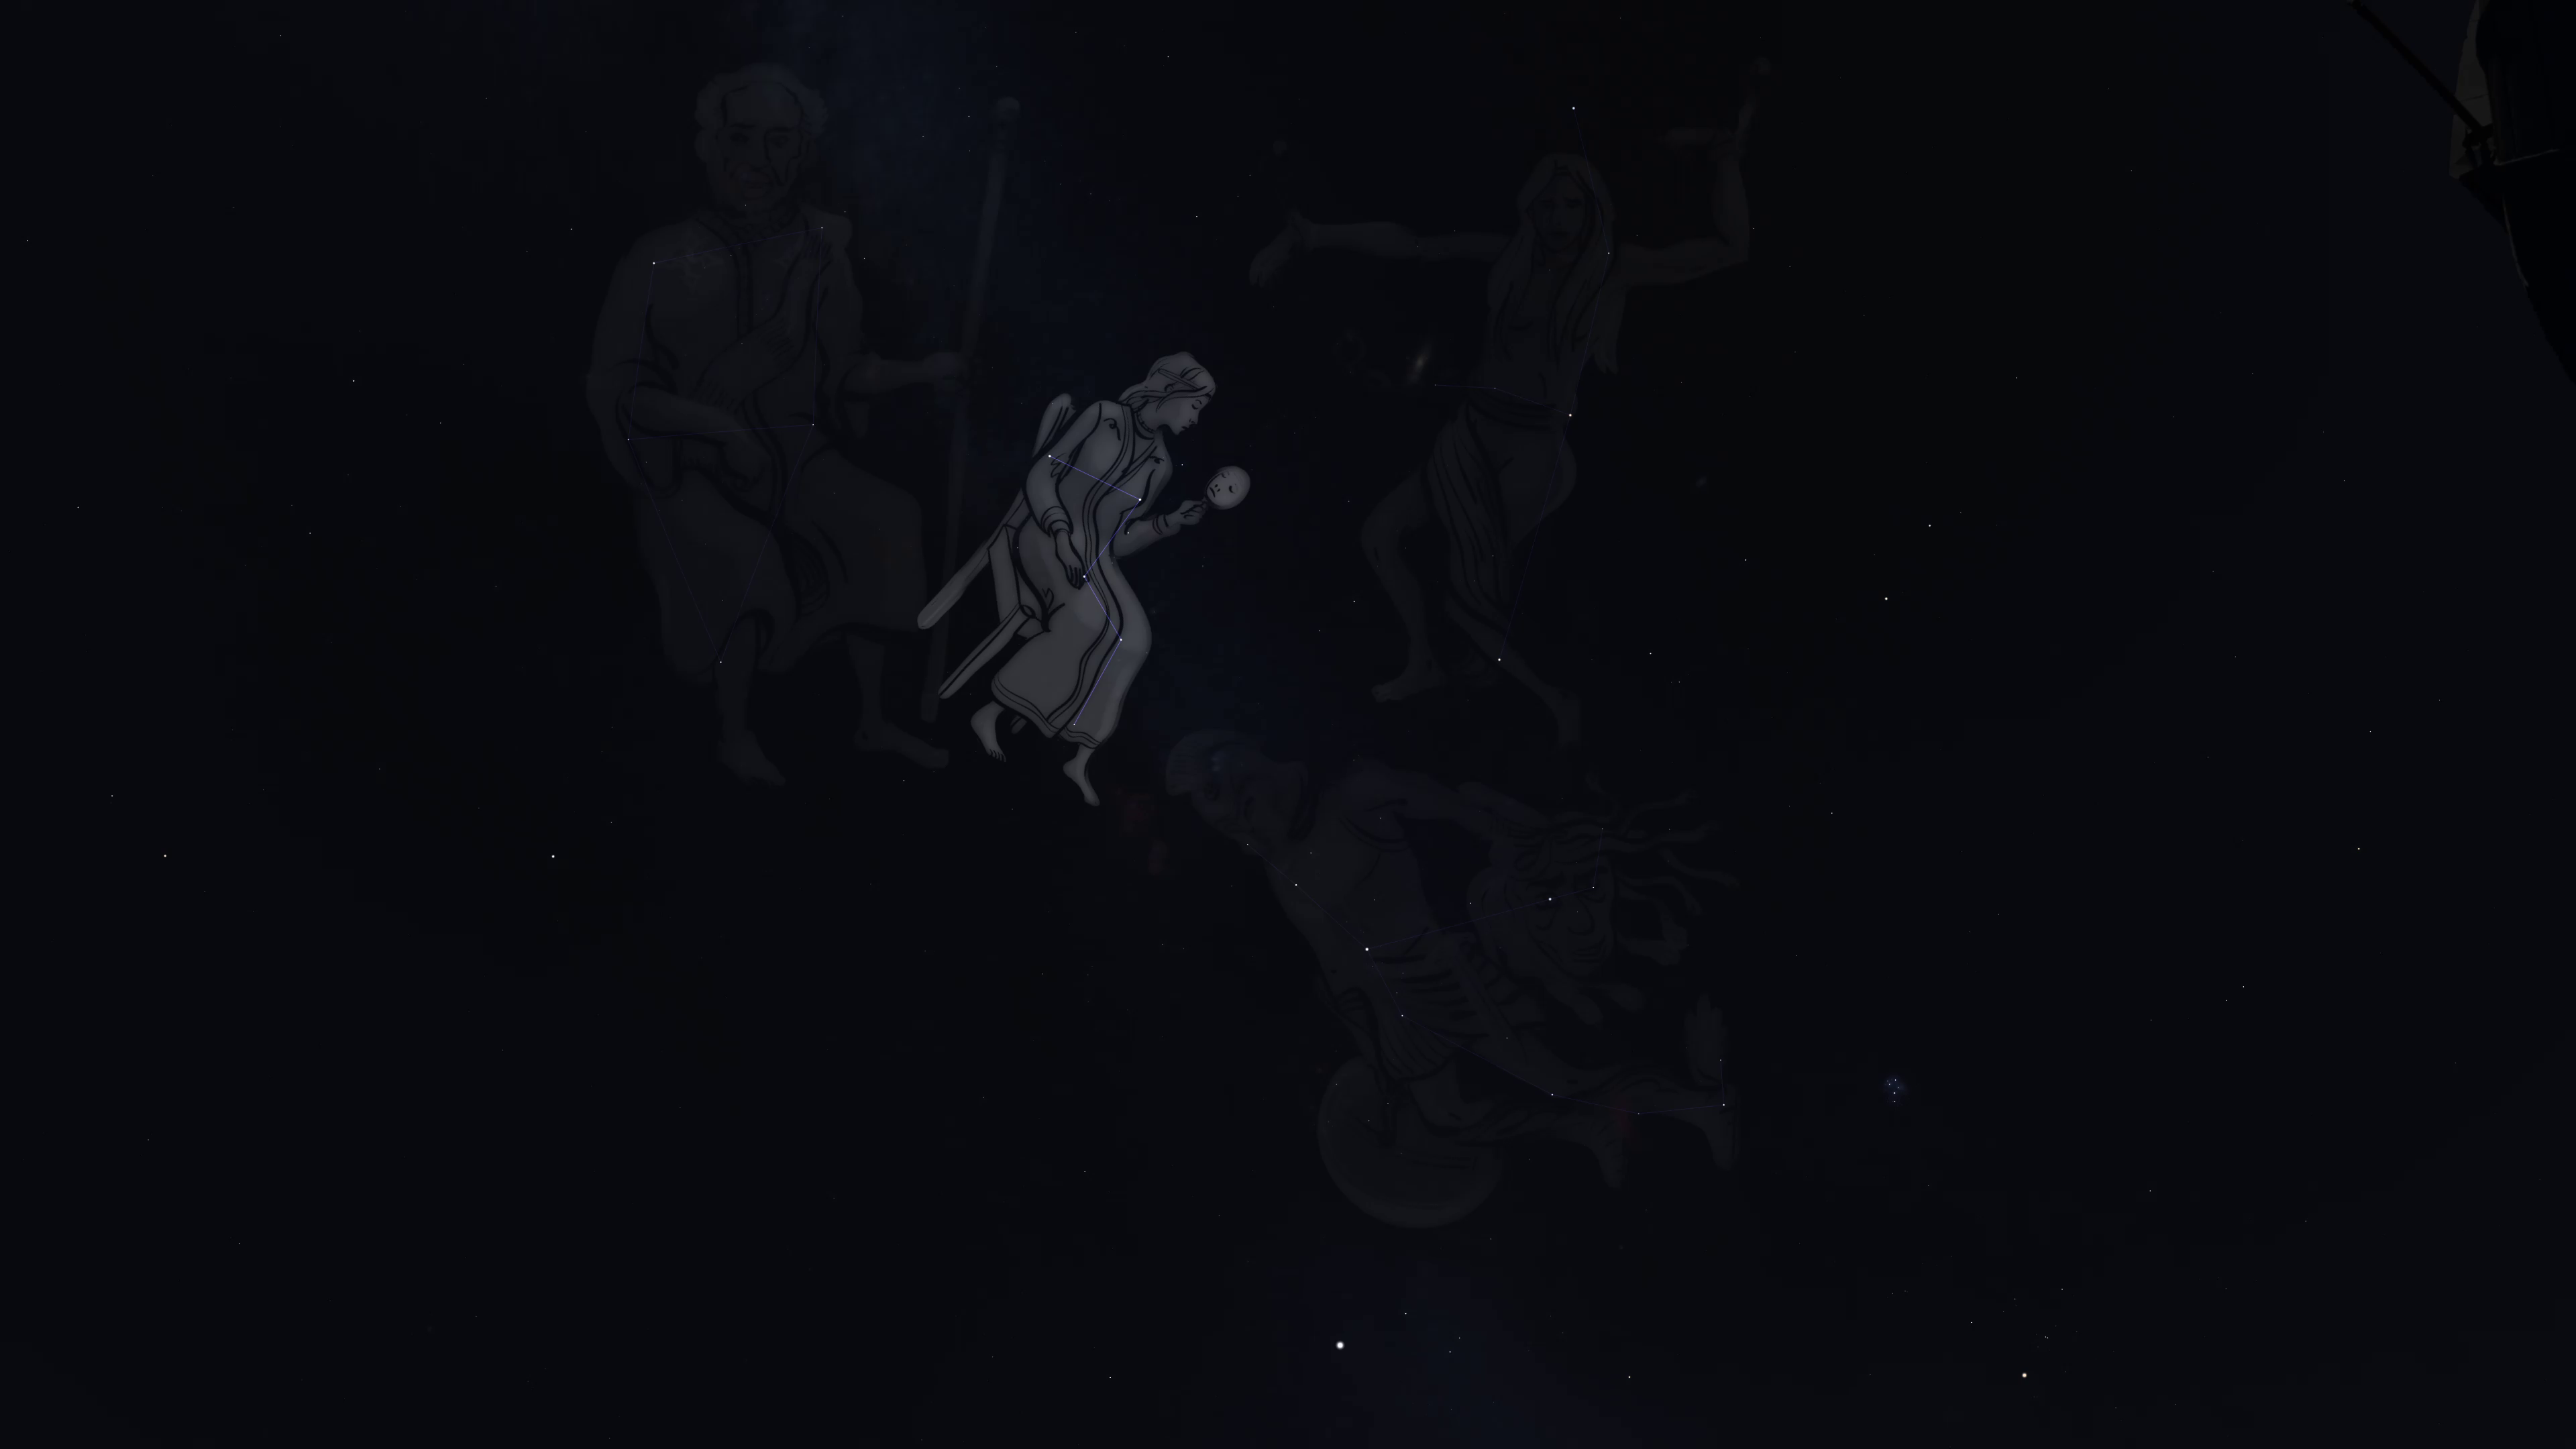
\includegraphics[width=.95\textwidth]{ac12_1.png}
	\caption{Demonstrace problematické scény z Prosincových Astronomických desetiminutovek.}\label{prac:ac12_1}
\end{figure}

Ačkoliv mi tento postup umožňoval větší kontrolu nad výsledným záběrem v editoru. Jeho nepraktičnost se ukázala v momentě, kdy jsem byl nucen scénu mírně pootočit kvůli chybě ve výpočtu data ve skriptu a byl jsem tedy nucen masku, kterou jsem již pečlivě naanimoval pro každé souhvězdí zvlášť během dalšího přechodu celou předělat.

V ten moment jsem se zamyslel, jestli by to nešlo udělat nějak lépe a napadlo mě, vyexportovat ze Stellaria jen potřebná souhvězdí a zbytek skrýt. Ukázalo se, že Stellarium má pro tento účel marker \textit{FlagIsolateSelected}, který umožní Stellariu renderovat pouze souhvězdí, která předem vyberu pomocí \textit{core.\-select\-Constellation\-By\-Name(name)}. Tato malá změna z pohledu diváka mi ušetřila nespočet hodin animování masek pro celé video. %chktex 36

Novinkou pro toto video byl také způsob zapracování objektů hlubokého vesmíru do jednotlivých záběrů. S tímto konceptem jsem si hrál i u zrušených říjnových Astronomických desetiminutovek, kde jsem dostal nápad, smíchat obrázky objektů hlubokého vesmíru s daty ze Stellaria. První snímek, který takto vznikl, můžete vidět jako obrázek~\ref{prac:ac12_2}. 

\begin{figure}[h]
	\centering
	\includegraphics[width=.95\textwidth]{ac12_2.png}
	\caption{První snímek s mixovanými objekty hlubokého vesmíru a dat ze stellaria, zpracování: Zoner Photo Studio X.}\label{prac:ac12_2}
\end{figure}

Tohoto efektu dosáhneme pomocí míchání metodou Lighten, kde zvolíme nejjasnější barvu každého pixelu z vrstev níže. Vstupní snímky, pokud se nejedná o snímky kulových hvězdokup, nejdříve zpracuji pomocí Starnet++, který ze snímků odstraní hvězdy. Následně vyčistím pozadí daného snímku, aby bylo co nejtmavší, jak je to možné. Tuto část snímku chceme odstranit a proto potřebujeme, aby ji metoda Lighten nikdy nevybrala, proto se snažím zajistit, aby měly tyto pixely co nejtmavší barvu. Následně do snímku vrátím některé hvězdy, které nezasahují do pozadí (Například u snímku~\ref{prac:ac12_2} bílého trpaslíka uprostřed mlhoviny M57).

Poslední krok je zarovnání snímku na místo, kde se na obloze nachází v realitě a pomalé prolnutí, využívající neschopnosti diváka všimnout si pomalých změn.

Tento typ zpracování obrázků dostal podporu od zbytku týmu a nyní ho využíváme pro většinu objektů hlubokého vesmíru.

Další výraznou novinkou bylo zahrnutí titulků do videa. Nejen že obsahují popisky
\end{document}
